% Chapter Template

\chapter{Extending Dose Transition Pathways for use in TITE-CRMs} % Main chapter title

\label{TITE-DTP} % For referencing this chapter elsewhere, use \ref{TITE-DTP}

%----------------------------------------------------------------------------------------
%	SECTION 1
%----------------------------------------------------------------------------------------

\section{Introduction}
\label{tite-dtp:Introduction}

Dose transition pathways (DTP), were developed as tool by Yap et al. \cite{yapDoseTransitionPathways2017} in order to address some of the issues around understanding and implementation of these complex and innovative designs, which were discussed in Chapter \ref{Chapter1}. DTPs can be considered a tool primarily for dose-finding trials where the primary objective is to determine a MTD (or TD\%\% at a specific target toxicity level) which is determined by the occurrence of DLTs recorded as a binary variable. The purpose of DTPs is to aid the design and analysis of these types of trials. This is done by projecting in advance the dose-escalation decisions for future cohorts based on data accrued. It can also be used as a calibration tool during the design phases of a trial to ascertain how the model behaves under certain outcomes and modify its specifications if necessary. These projections can then be visualised and help illustrate how the model operates and communicate possible future decisions that may be made. 

In the paper by Yap et al. \cite{yapDoseTransitionPathways2017}, DTPs are introduced through their illustrative use in a trial with a CRM design. They discuss that the idea of DTPs can be extended to other model-based designs such as the TITE-CRM and phase\RN{1}/\RN{2} designs that consider efficacy and toxicity. DTPs are produced based on the outcome data collected and for both of these possible extensions the outcome data is slightly more complex which makes producing DTPs for these designs challenging. Specifically, for the TITE-CRM additional data is needed dependent on if the patient is to be fully or partially weighted. That is if the patient has not experienced a DLT they will be partially weighted in the model based on the time they have spent in the trial. This makes mapping out dose-escalation decisions difficult since we are no longer dealing with a simple binary variable of DLT/no DLT. 

In this chapter we aim to explore the potential of extending DTPs for use in TITE-CRMs. We start by providing an example of a DTP for a simple CRM design to better understand what they are and how they can be used. We then look at some of the issues with extending DTPs to TITE-CRMs and present possible solutions for how they may be overcome.


%----------------------------------------------------------------------------------------
%	SECTION 2
%----------------------------------------------------------------------------------------

\section{Dose Transition Pathways}
\label{tite-dtp:DTPs}

In order to explore how DTPs can be extended for use in TITE-CRMs we first look at how they would be used for a simple CRM trial. To do this we look at how CRM designs are implemented and analysed and how DTPs can be incorporated in these processes. 

When implementing a CRM design multiple parameters need to be considered and specified. These are: number of doses, target toxicity level, dose-toxicity model, dose-toxicity skeleton, method of inference, decision rules, sample size, cohort size, safety modifications, and stopping rules \cite{wheelerHowDesignDosefinding2019}. This usually requires the input from multiple sources such as the statistician, clinician and trial management team. Typically, once these parameters have been specified, simulations can be run for various clinically relevant scenarios to obtain operating characteristics for the specified CRM design. At this point these results can be reassessed and the specifications of the CRM can be updated  and this whole process can be repeated until an acceptable design is reached. 

Even after multiple rounds of simulations there is still the risk that a statistically optimal design may not be optimal in practice. This could be due to the scenarios used in simulations not being representative of what is observed during the running of the trial. This may also occur when model recommendations are deemed clinically inexplicable and dose-escalation decisions recommended by the model are ignored or overruled. Whilst dose recommendations from the model should be used as guidance, if its recommendations are constantly being ignored it undermines the model and brings into question it's specifications. DTPs can be used to avoid this from occurring and can help calibrate the model, by providing insight during the design phase of the trial into what recommendations the model is making. This will help clinicians as well as statisticians better understand how the model works and calibrate it accordingly so clinically reasonable decisions are being made.   

DTPs can also be utilised during the analysis of a trial. In a 3+3 trial just by knowing the rules of the design we already know what dose-escalation decision will be made for all possible outcomes of one cohort. If zero out of three patients (0/3) experience a DLT we escalate to the next highest dose; if one out of three patients (1/3) experiences a DLT we recruit a further 3 patients to the same dose-level; and if two out of three (2/3) patients experience a DLT we de-escalate to a lower dose or stop the trial if already at the lowest dose. This can be done and computed without the need of a statistician. On the other hand, we have designs such as the CRM where this is not as simple since the next recommended dose will be based on the accrued data. Here DTPs can be utilised and present this information by analysing all possible outcomes and presenting the dose recommendations these lead to.

The number of pathways can be calculated using the number of cohorts ($x$) and the number of patients in each cohort ($y$). Here, the total sample size is $xy$ and the number of pathways is $(y+1)^x$. So, for a trial recruiting 10 cohorts of 3 patients the number of pathways would be over 1 million ($[3+1]^{10} = 1,048,576$). It is possible that there may be less pathways based on any stopping rules which cause the trial to stop early. Obviously, presenting this many pathways is difficult and may also be unintuitive. Yap et al. \cite{yapDoseTransitionPathways2017} suggest using the first group of cohorts to help facilitate discussion with investigators during the design phase of the trial. DTPs can also be updated during dose-escalation phases as well by incorporating the accrued data then projecting pathways for subsequent cohorts. In the next section, section \ref{tite-dtp:Example-DTPs} we provide a generic trial example to show how DTPs can be implemented.  

%-----------------------------------
%	SUBSECTION 1
%-----------------------------------
\subsection{Example trial to illustrate DTPs}
\label{tite-dtp:Example-DTPs}

Lets consider an early phase trial aiming to determine the TD25 of a single agent, Table \ref{tab_tite-dtp:exampleCRMspecs} details all the parameters we need to set-up the CRM design. First we specify the clinical parameters; there will be 5 dose levels ($d_1$, ... ,$d_5$), the trial will start at dose-level 2 ($d_2$), the target sample size will be 30 patients, patients will be recruited in cohorts of 3 (10 cohorts overall) and the target DLT rate will be 25\% (TD25). A single-stage CRM will be used with a power model to model the dose-toxicity curve, Bayesian estimation methods will also be used. Initial guesses for the DLT rates are specified as 0.04, 0.08, 0.16, 0.25 and 0.35 for dose-levels 1-5 respectively, this assumes dose-level 4 ($d_4$) will be the TD25. 

\begin{table}[h!]
	\centering
	\caption{Specification of parameters for an example CRM trial. }
	\label{tab_tite-dtp:exampleCRMspecs}
	\begin{tabular}{l|c}
		\hline
		\textbf{Parmaeter}     & \textbf{Value}               \\ \hline
		Number of dose-levels  & 5                            \\
		Starting dose-level    & 2                            \\
		Sample size            & 30                           \\
		Cohort size            & 3                            \\
		Target DLT rate        & 25\%                         \\
		Dose-toxicity model    & Power model                  \\
		Dose-toxicity skeleton & 0.04, 0.08, 0.16, 0.25, 0.35 \\
		Method of inference    & Bayesian                     \\ \hline
	\end{tabular}
\end{table}

We assume the prior distribution for the slope parameter in the power model will be normally distributed with a mean of 0 and variance of 1.34. This prior distribution was chosen due to convention. These values are based on work by O'Quigley and Shen \cite{oquigleyContinualReassessmentMethod1996} that proposed a suitable prior distribution would be a normal distribution with a mean of 0 and a sufficiently large variance, they go on to use a variance of 1.34 which was adopted by others and eventually became the norm. As this example is for only illustrative purposes and given its simplicity we feel these are adequate choices. Wheeler et al \cite{wheelerHowDesignDosefinding2019} also discuss choices of prior parameters when designing a dose-finding study, obviously in practice more thought should be given to the selection of all parameters. 

Most of the parameter specifications made here are fairly arbitrary, in practice these specifications should have either a clinical or statistical rationale behind them based on the context of the trial which requires input from multiple parties. Once an initial set of these parameters have been selected, it's usually at this stage that simulations take place in order to assess the operating characteristics of the design under various scenarios. At this point DTPs can also be generated. 

%-----------------------------------
%	SUBSECTION 2
%-----------------------------------
\subsection{Using DTPs to calibrate the CRM}
\label{tite-dtp:UsingDTPs-Calibration}

Since we have specified a sample size of 30 and cohort size of 3 that means we will have 10 cohorts and therefore 1,048,576 pathways ($[3+1]^{10} = 1,048,576$). Patients in each cohort are considered to either experience a toxic event (T) or have no toxic event (N). For the first cohort of three patients there are four possible outcomes: all patients in experience no toxicity (NNN), one patients experience a toxic event (NNT), two patients experience a toxic event (NTT) and all three patients experience a toxic event (TTT). For the subsequent cohort the same set of 4 outcomes can be observed but then in combination with the previous cohort this creates 16 different outcomes for the first 2 cohorts (6 patients). This process is then continued for each cohort creating exponentially more pathways. 

Given the impracticalities of presenting and summarising all these pathways we can instead present the pathways of the first three cohorts of patients. In this case there are only 64 potential pathways ($[3+1]^{3} = 64$). Table \ref{tab_tite-dtp:InitialDTPExample} lists all the potential pathways for the first three cohorts of patients. Similarly, we can also represent these pathways visually using either a node plot (Figure \ref{fig_tite-dtp:InitialDTPExampleNode}, generated using the R package escalation \cite{brockModularApproachDose2020}). Originally, when DTPs were first introduced, a flow plot was used to visualise the pathways. These have also been produced (Figure \ref{fig_tite-dtp:InitialDTPExampleFlow}, generated using the R package dtpcrm \cite{yapDtpcrmDoseTransition2019}) but due to limitations with the software they only show the pathways for the first two cohorts. 

\begin{table}[H]
	
	\caption{\label{tab_tite-dtp:InitialDTPExample}Initial DTP for the first three cohorts of our example CRM.}
	\centering
	\resizebox{\linewidth}{!}{
		\fontsize{4}{3}\selectfont
		\begin{tabular}[t]{cccccccc}
			\toprule
			\multicolumn{1}{c}{} & \multicolumn{2}{c}{Cohort 1} & \multicolumn{2}{c}{Cohort 2} & \multicolumn{2}{c}{Cohort 3} & \multicolumn{1}{c}{Cohort 4} \\
			\cmidrule(l{3pt}r{3pt}){2-3} \cmidrule(l{3pt}r{3pt}){4-5} \cmidrule(l{3pt}r{3pt}){6-7} \cmidrule(l{3pt}r{3pt}){8-8}
			Pathway & Dose & Outcomes & Dose & Outcomes & Dose & Outcomes & Dose\\
			\midrule
			\cellcolor{gray!6}{1} & \cellcolor{gray!6}{2} & \cellcolor{gray!6}{NNN} & \cellcolor{gray!6}{5} & \cellcolor{gray!6}{NNN} & \cellcolor{gray!6}{5} & \cellcolor{gray!6}{NNN} & \cellcolor{gray!6}{5}\\
			2 & 2 & NNN & 5 & NNN & 5 & NNT & 5\\
			\cellcolor{gray!6}{3} & \cellcolor{gray!6}{2} & \cellcolor{gray!6}{NNN} & \cellcolor{gray!6}{5} & \cellcolor{gray!6}{NNN} & \cellcolor{gray!6}{5} & \cellcolor{gray!6}{NTT} & \cellcolor{gray!6}{4}\\
			4 & 2 & NNN & 5 & NNN & 5 & TTT & 3\\
			\cellcolor{gray!6}{5} & \cellcolor{gray!6}{2} & \cellcolor{gray!6}{NNN} & \cellcolor{gray!6}{5} & \cellcolor{gray!6}{NNT} & \cellcolor{gray!6}{5} & \cellcolor{gray!6}{NNN} & \cellcolor{gray!6}{5}\\
			6 & 2 & NNN & 5 & NNT & 5 & NNT & 4\\
			\cellcolor{gray!6}{7} & \cellcolor{gray!6}{2} & \cellcolor{gray!6}{NNN} & \cellcolor{gray!6}{5} & \cellcolor{gray!6}{NNT} & \cellcolor{gray!6}{5} & \cellcolor{gray!6}{NTT} & \cellcolor{gray!6}{3}\\
			8 & 2 & NNN & 5 & NNT & 5 & TTT & 2\\
			\cellcolor{gray!6}{9} & \cellcolor{gray!6}{2} & \cellcolor{gray!6}{NNN} & \cellcolor{gray!6}{5} & \cellcolor{gray!6}{NTT} & \cellcolor{gray!6}{3} & \cellcolor{gray!6}{NNN} & \cellcolor{gray!6}{4}\\
			10 & 2 & NNN & 5 & NTT & 3 & NNT & 3\\
			\cellcolor{gray!6}{11} & \cellcolor{gray!6}{2} & \cellcolor{gray!6}{NNN} & \cellcolor{gray!6}{5} & \cellcolor{gray!6}{NTT} & \cellcolor{gray!6}{3} & \cellcolor{gray!6}{NTT} & \cellcolor{gray!6}{2}\\
			12 & 2 & NNN & 5 & NTT & 3 & TTT & 1\\
			\cellcolor{gray!6}{13} & \cellcolor{gray!6}{2} & \cellcolor{gray!6}{NNN} & \cellcolor{gray!6}{5} & \cellcolor{gray!6}{TTT} & \cellcolor{gray!6}{2} & \cellcolor{gray!6}{NNN} & \cellcolor{gray!6}{3}\\
			14 & 2 & NNN & 5 & TTT & 2 & NNT & 2\\
			\cellcolor{gray!6}{15} & \cellcolor{gray!6}{2} & \cellcolor{gray!6}{NNN} & \cellcolor{gray!6}{5} & \cellcolor{gray!6}{TTT} & \cellcolor{gray!6}{2} & \cellcolor{gray!6}{NTT} & \cellcolor{gray!6}{1}\\
			16 & 2 & NNN & 5 & TTT & 2 & TTT & 1\\
			\cellcolor{gray!6}{17} & \cellcolor{gray!6}{2} & \cellcolor{gray!6}{NNT} & \cellcolor{gray!6}{2} & \cellcolor{gray!6}{NNN} & \cellcolor{gray!6}{3} & \cellcolor{gray!6}{NNN} & \cellcolor{gray!6}{4}\\
			18 & 2 & NNT & 2 & NNN & 3 & NNT & 3\\
			\cellcolor{gray!6}{19} & \cellcolor{gray!6}{2} & \cellcolor{gray!6}{NNT} & \cellcolor{gray!6}{2} & \cellcolor{gray!6}{NNN} & \cellcolor{gray!6}{3} & \cellcolor{gray!6}{NTT} & \cellcolor{gray!6}{2}\\
			20 & 2 & NNT & 2 & NNN & 3 & TTT & 1\\
			\cellcolor{gray!6}{21} & \cellcolor{gray!6}{2} & \cellcolor{gray!6}{NNT} & \cellcolor{gray!6}{2} & \cellcolor{gray!6}{NNT} & \cellcolor{gray!6}{1} & \cellcolor{gray!6}{NNN} & \cellcolor{gray!6}{2}\\
			22 & 2 & NNT & 2 & NNT & 1 & NNT & 1\\
			\cellcolor{gray!6}{23} & \cellcolor{gray!6}{2} & \cellcolor{gray!6}{NNT} & \cellcolor{gray!6}{2} & \cellcolor{gray!6}{NNT} & \cellcolor{gray!6}{1} & \cellcolor{gray!6}{NTT} & \cellcolor{gray!6}{1}\\
			24 & 2 & NNT & 2 & NNT & 1 & TTT & 1\\
			\cellcolor{gray!6}{25} & \cellcolor{gray!6}{2} & \cellcolor{gray!6}{NNT} & \cellcolor{gray!6}{2} & \cellcolor{gray!6}{NTT} & \cellcolor{gray!6}{1} & \cellcolor{gray!6}{NNN} & \cellcolor{gray!6}{1}\\
			26 & 2 & NNT & 2 & NTT & 1 & NNT & 1\\
			\cellcolor{gray!6}{27} & \cellcolor{gray!6}{2} & \cellcolor{gray!6}{NNT} & \cellcolor{gray!6}{2} & \cellcolor{gray!6}{NTT} & \cellcolor{gray!6}{1} & \cellcolor{gray!6}{NTT} & \cellcolor{gray!6}{1}\\
			28 & 2 & NNT & 2 & NTT & 1 & TTT & 1\\
			\cellcolor{gray!6}{29} & \cellcolor{gray!6}{2} & \cellcolor{gray!6}{NNT} & \cellcolor{gray!6}{2} & \cellcolor{gray!6}{TTT} & \cellcolor{gray!6}{1} & \cellcolor{gray!6}{NNN} & \cellcolor{gray!6}{1}\\
			30 & 2 & NNT & 2 & TTT & 1 & NNT & 1\\
			\cellcolor{gray!6}{31} & \cellcolor{gray!6}{2} & \cellcolor{gray!6}{NNT} & \cellcolor{gray!6}{2} & \cellcolor{gray!6}{TTT} & \cellcolor{gray!6}{1} & \cellcolor{gray!6}{NTT} & \cellcolor{gray!6}{1}\\
			32 & 2 & NNT & 2 & TTT & 1 & TTT & 1\\
			\cellcolor{gray!6}{33} & \cellcolor{gray!6}{2} & \cellcolor{gray!6}{NTT} & \cellcolor{gray!6}{1} & \cellcolor{gray!6}{NNN} & \cellcolor{gray!6}{1} & \cellcolor{gray!6}{NNN} & \cellcolor{gray!6}{2}\\
			34 & 2 & NTT & 1 & NNN & 1 & NNT & 1\\
			\cellcolor{gray!6}{35} & \cellcolor{gray!6}{2} & \cellcolor{gray!6}{NTT} & \cellcolor{gray!6}{1} & \cellcolor{gray!6}{NNN} & \cellcolor{gray!6}{1} & \cellcolor{gray!6}{NTT} & \cellcolor{gray!6}{1}\\
			36 & 2 & NTT & 1 & NNN & 1 & TTT & 1\\
			\cellcolor{gray!6}{37} & \cellcolor{gray!6}{2} & \cellcolor{gray!6}{NTT} & \cellcolor{gray!6}{1} & \cellcolor{gray!6}{NNT} & \cellcolor{gray!6}{1} & \cellcolor{gray!6}{NNN} & \cellcolor{gray!6}{1}\\
			38 & 2 & NTT & 1 & NNT & 1 & NNT & 1\\
			\cellcolor{gray!6}{39} & \cellcolor{gray!6}{2} & \cellcolor{gray!6}{NTT} & \cellcolor{gray!6}{1} & \cellcolor{gray!6}{NNT} & \cellcolor{gray!6}{1} & \cellcolor{gray!6}{NTT} & \cellcolor{gray!6}{1}\\
			40 & 2 & NTT & 1 & NNT & 1 & TTT & 1\\
			\cellcolor{gray!6}{41} & \cellcolor{gray!6}{2} & \cellcolor{gray!6}{NTT} & \cellcolor{gray!6}{1} & \cellcolor{gray!6}{NTT} & \cellcolor{gray!6}{1} & \cellcolor{gray!6}{NNN} & \cellcolor{gray!6}{1}\\
			42 & 2 & NTT & 1 & NTT & 1 & NNT & 1\\
			\cellcolor{gray!6}{43} & \cellcolor{gray!6}{2} & \cellcolor{gray!6}{NTT} & \cellcolor{gray!6}{1} & \cellcolor{gray!6}{NTT} & \cellcolor{gray!6}{1} & \cellcolor{gray!6}{NTT} & \cellcolor{gray!6}{1}\\
			44 & 2 & NTT & 1 & NTT & 1 & TTT & 1\\
			\cellcolor{gray!6}{45} & \cellcolor{gray!6}{2} & \cellcolor{gray!6}{NTT} & \cellcolor{gray!6}{1} & \cellcolor{gray!6}{TTT} & \cellcolor{gray!6}{1} & \cellcolor{gray!6}{NNN} & \cellcolor{gray!6}{1}\\
			46 & 2 & NTT & 1 & TTT & 1 & NNT & 1\\
			\cellcolor{gray!6}{47} & \cellcolor{gray!6}{2} & \cellcolor{gray!6}{NTT} & \cellcolor{gray!6}{1} & \cellcolor{gray!6}{TTT} & \cellcolor{gray!6}{1} & \cellcolor{gray!6}{NTT} & \cellcolor{gray!6}{1}\\
			48 & 2 & NTT & 1 & TTT & 1 & TTT & 1\\
			\cellcolor{gray!6}{49} & \cellcolor{gray!6}{2} & \cellcolor{gray!6}{TTT} & \cellcolor{gray!6}{1} & \cellcolor{gray!6}{NNN} & \cellcolor{gray!6}{1} & \cellcolor{gray!6}{NNN} & \cellcolor{gray!6}{1}\\
			50 & 2 & TTT & 1 & NNN & 1 & NNT & 1\\
			\cellcolor{gray!6}{51} & \cellcolor{gray!6}{2} & \cellcolor{gray!6}{TTT} & \cellcolor{gray!6}{1} & \cellcolor{gray!6}{NNN} & \cellcolor{gray!6}{1} & \cellcolor{gray!6}{NTT} & \cellcolor{gray!6}{1}\\
			52 & 2 & TTT & 1 & NNN & 1 & TTT & 1\\
			\cellcolor{gray!6}{53} & \cellcolor{gray!6}{2} & \cellcolor{gray!6}{TTT} & \cellcolor{gray!6}{1} & \cellcolor{gray!6}{NNT} & \cellcolor{gray!6}{1} & \cellcolor{gray!6}{NNN} & \cellcolor{gray!6}{1}\\
			54 & 2 & TTT & 1 & NNT & 1 & NNT & 1\\
			\cellcolor{gray!6}{55} & \cellcolor{gray!6}{2} & \cellcolor{gray!6}{TTT} & \cellcolor{gray!6}{1} & \cellcolor{gray!6}{NNT} & \cellcolor{gray!6}{1} & \cellcolor{gray!6}{NTT} & \cellcolor{gray!6}{1}\\
			56 & 2 & TTT & 1 & NNT & 1 & TTT & 1\\
			\cellcolor{gray!6}{57} & \cellcolor{gray!6}{2} & \cellcolor{gray!6}{TTT} & \cellcolor{gray!6}{1} & \cellcolor{gray!6}{NTT} & \cellcolor{gray!6}{1} & \cellcolor{gray!6}{NNN} & \cellcolor{gray!6}{1}\\
			58 & 2 & TTT & 1 & NTT & 1 & NNT & 1\\
			\cellcolor{gray!6}{59} & \cellcolor{gray!6}{2} & \cellcolor{gray!6}{TTT} & \cellcolor{gray!6}{1} & \cellcolor{gray!6}{NTT} & \cellcolor{gray!6}{1} & \cellcolor{gray!6}{NTT} & \cellcolor{gray!6}{1}\\
			60 & 2 & TTT & 1 & NTT & 1 & TTT & 1\\
			\cellcolor{gray!6}{61} & \cellcolor{gray!6}{2} & \cellcolor{gray!6}{TTT} & \cellcolor{gray!6}{1} & \cellcolor{gray!6}{TTT} & \cellcolor{gray!6}{1} & \cellcolor{gray!6}{NNN} & \cellcolor{gray!6}{1}\\
			62 & 2 & TTT & 1 & TTT & 1 & NNT & 1\\
			\cellcolor{gray!6}{63} & \cellcolor{gray!6}{2} & \cellcolor{gray!6}{TTT} & \cellcolor{gray!6}{1} & \cellcolor{gray!6}{TTT} & \cellcolor{gray!6}{1} & \cellcolor{gray!6}{NTT} & \cellcolor{gray!6}{1}\\
			64 & 2 & TTT & 1 & TTT & 1 & TTT & 1\\
			\bottomrule
	\end{tabular}}
\end{table}

\begin{figure}[h!]
	\centering
	\caption[Initial DTP node plot.]{Initial DTP node plot for the first three cohorts of our example CRM.}
	\label{fig_tite-dtp:InitialDTPExampleNode}
	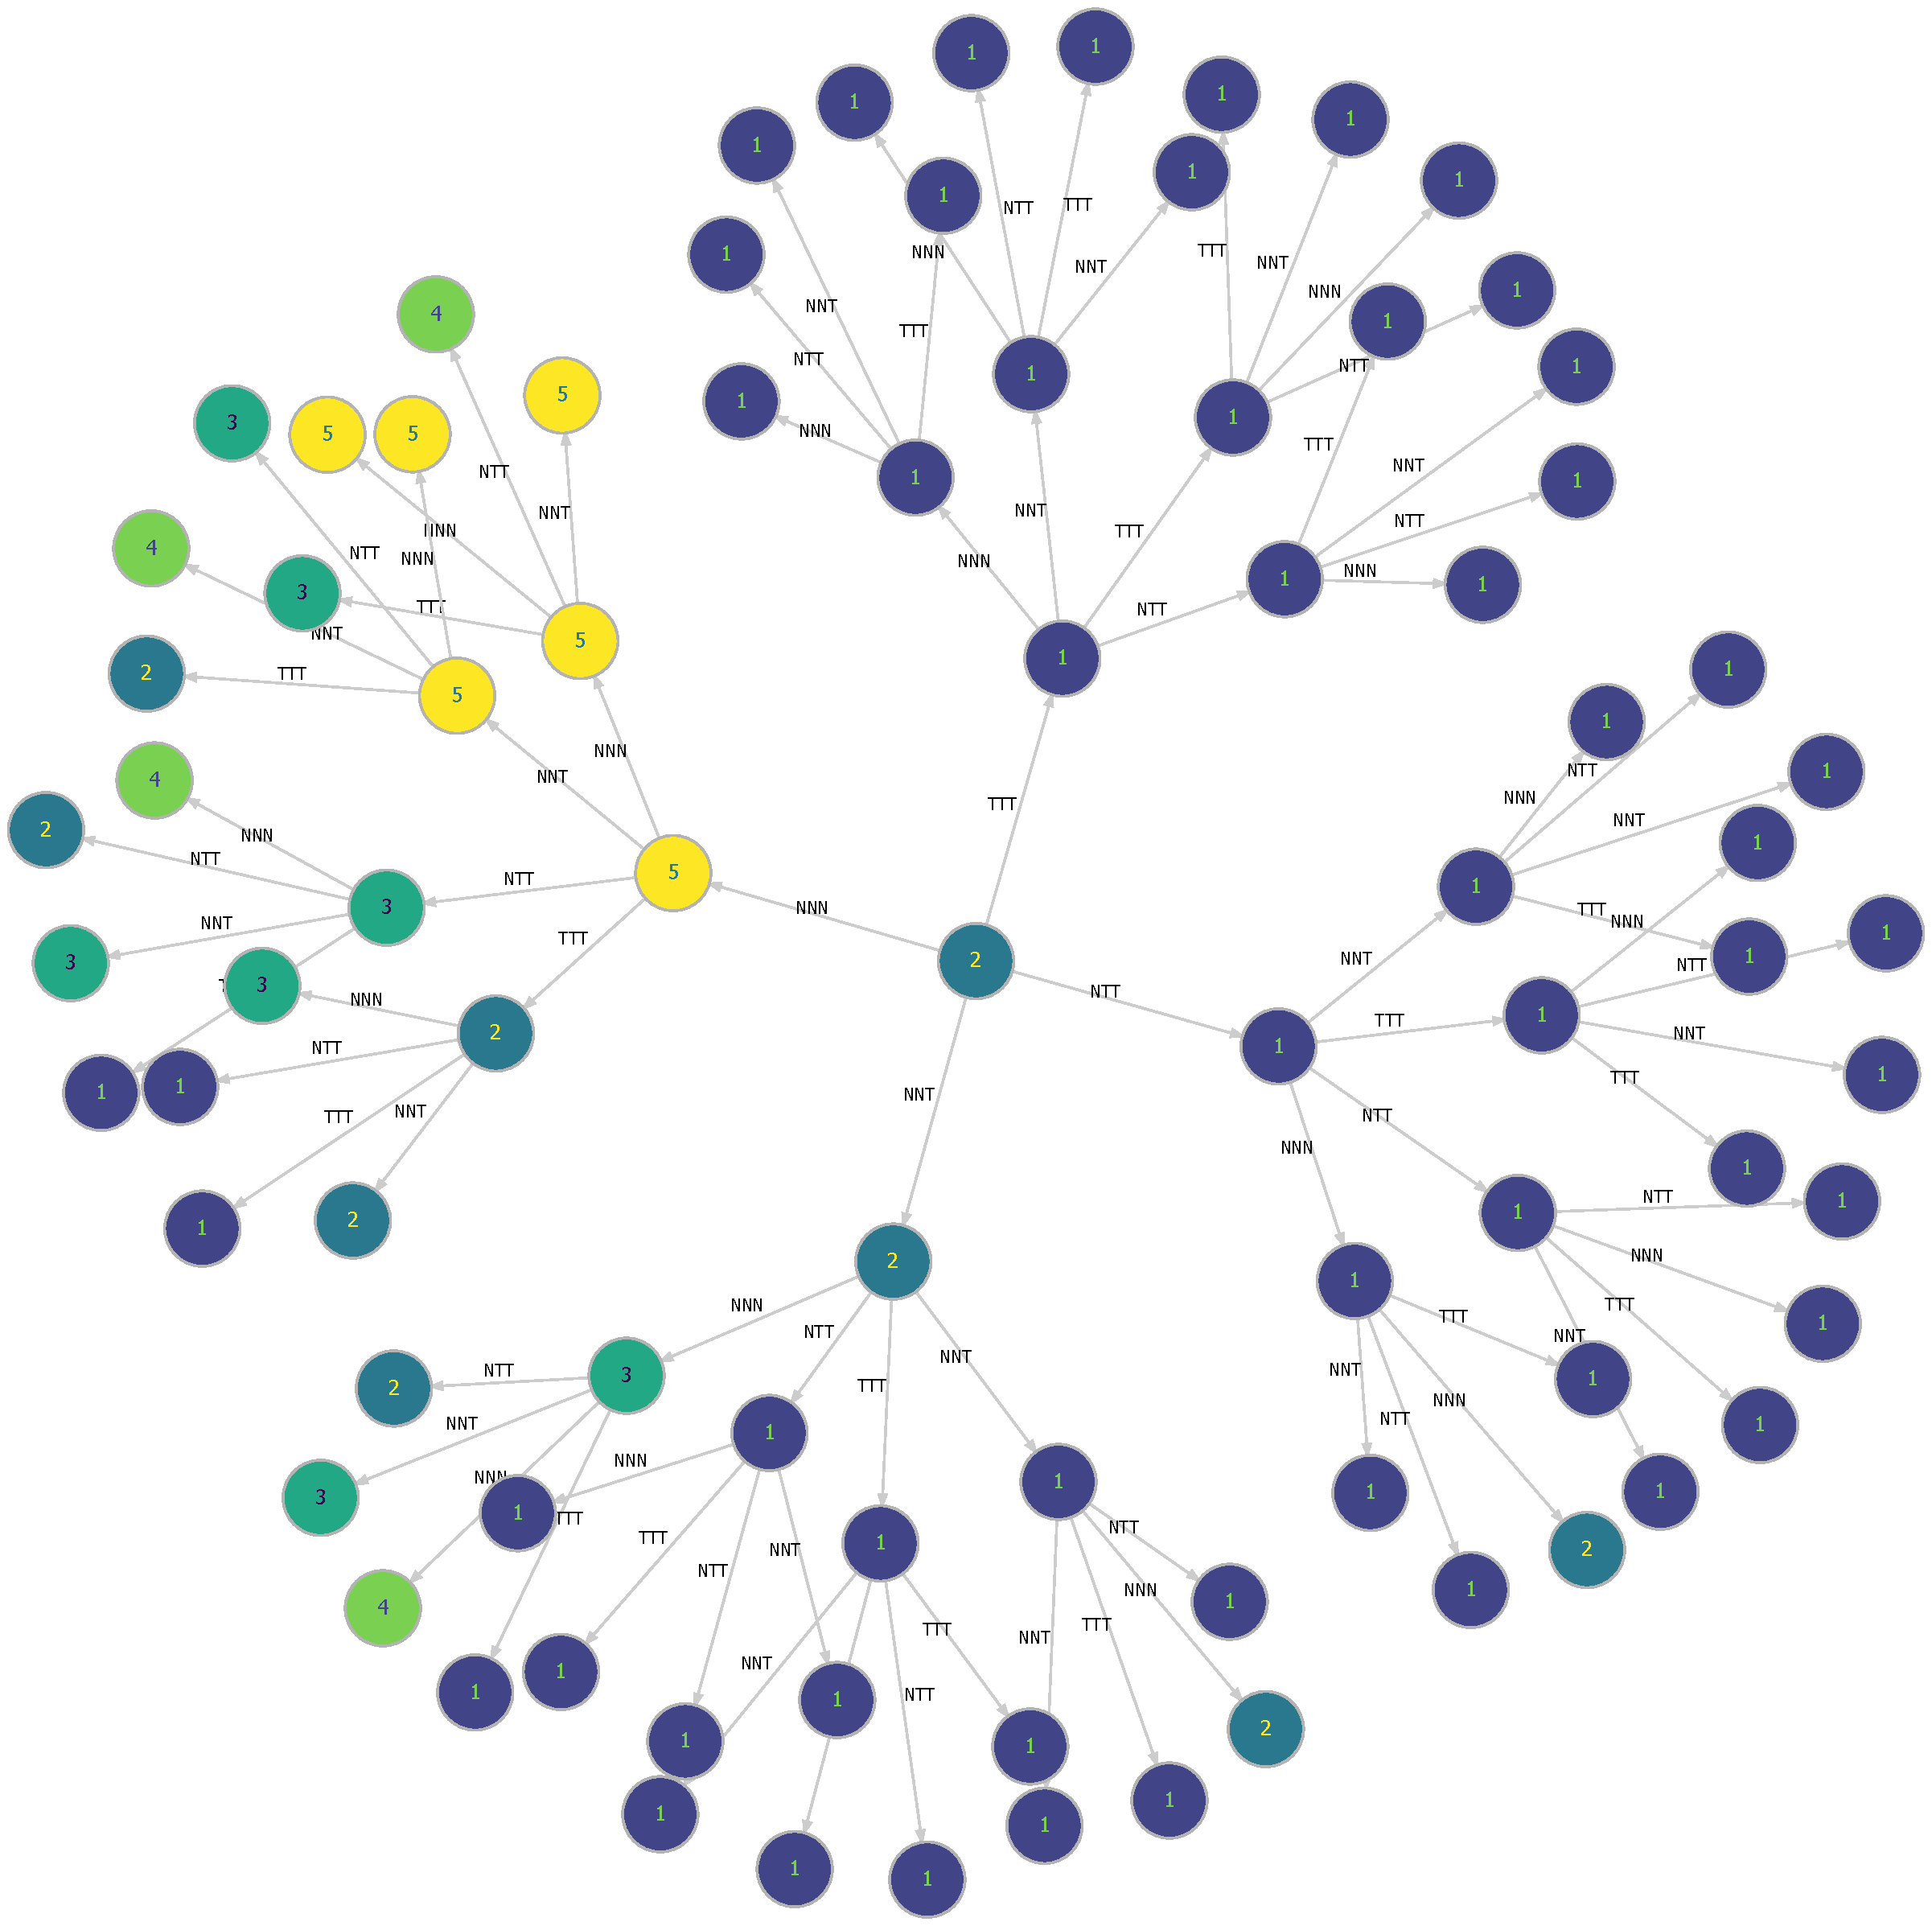
\includegraphics[width=\textwidth]{TITE-DTP-InitialExampleDTPNode}
\end{figure}

\begin{figure}[h!]
	\centering
	\caption[Initial DTP flow plot.]{Node plot of the initial DTP for the first two cohorts of our example CRM.}
	\label{fig_tite-dtp:InitialDTPExampleFlow}
	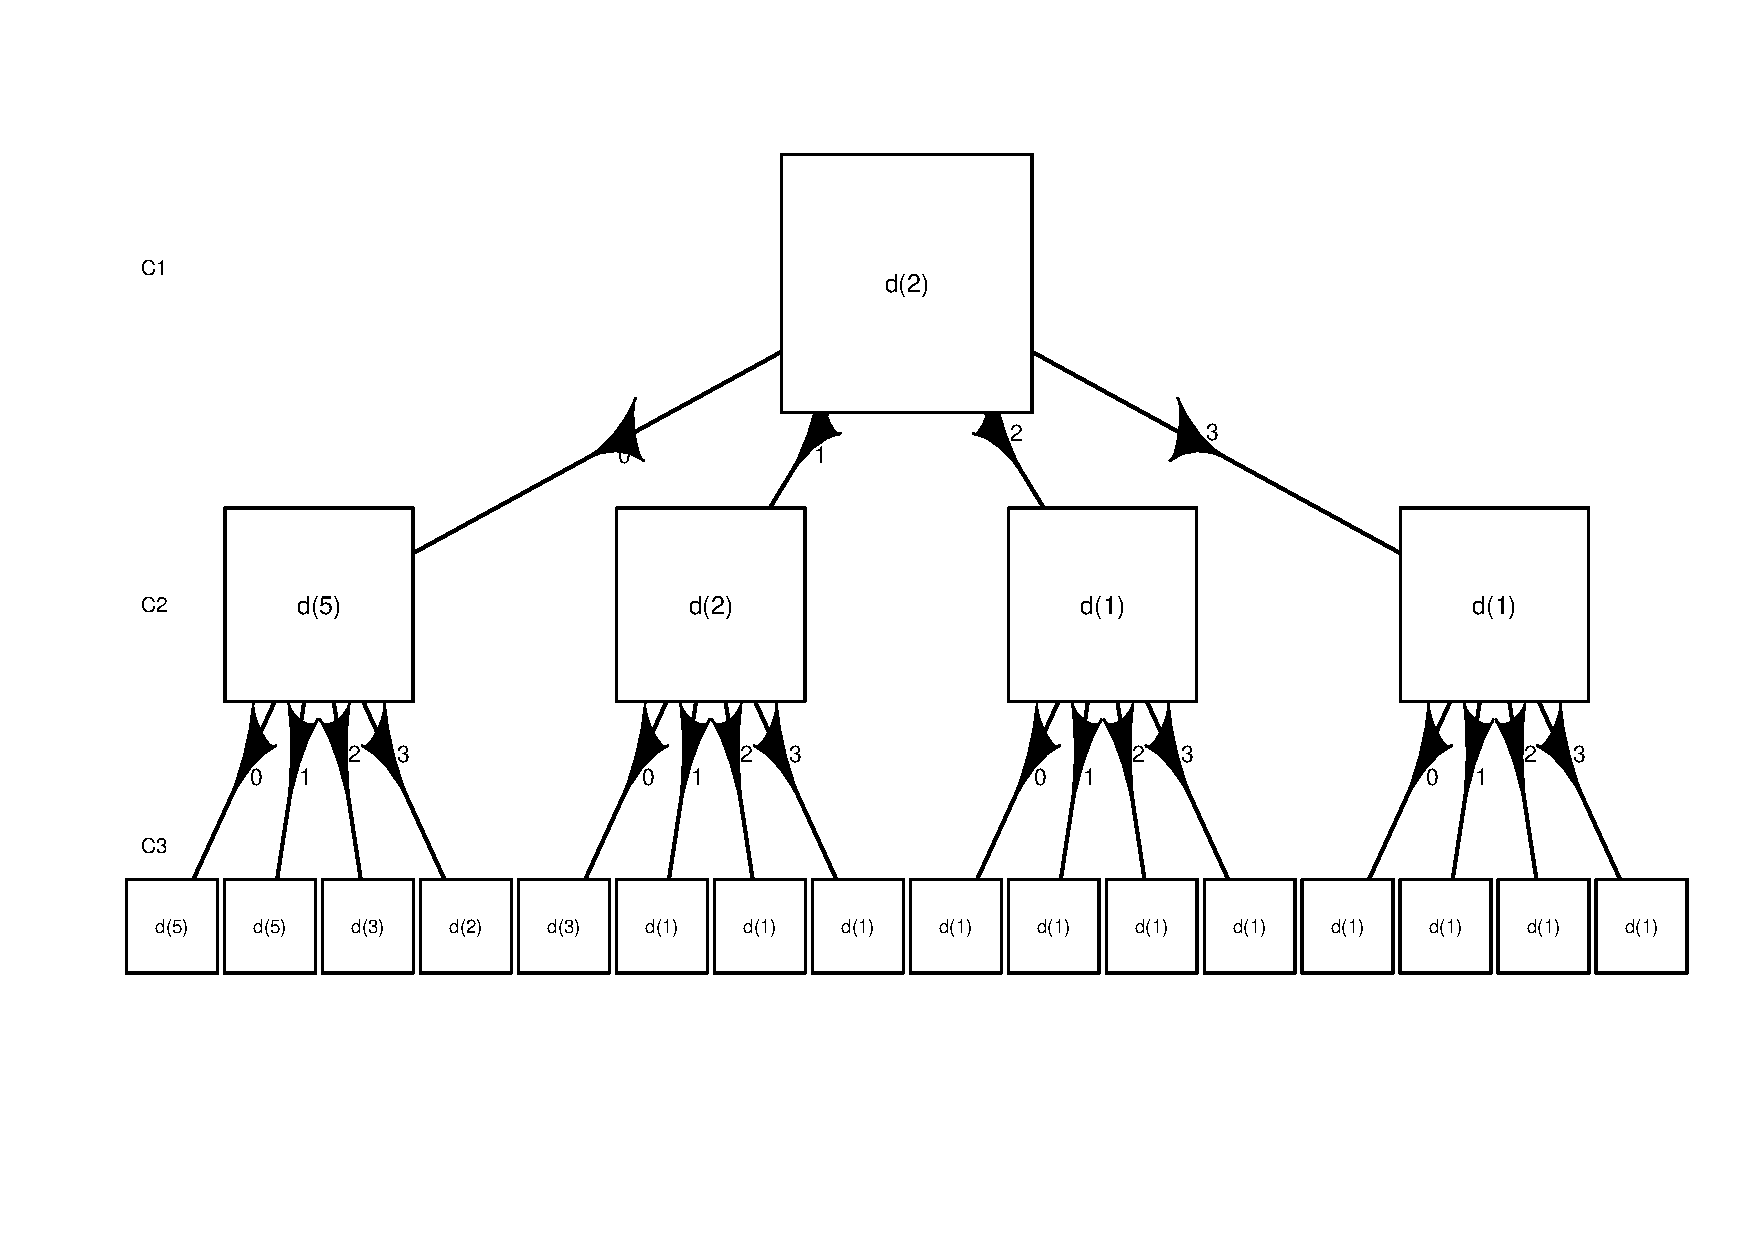
\includegraphics[width=\textwidth]{TITE-DTP-InitialExampleDTPFlow}
\end{figure}

From Table \ref{tab_tite-dtp:InitialDTPExample}, looking at pathways 33-64, we can see that if there are two or more toxicities in the first cohort the CRM will always de-escalate the dose and if there are one or more toxicities in the next two cohorts it will stay at dose-level 1. We can also see from pathways 17-32 if we observe a toxicity in the first cohort we will stay at the same dose-level for the next cohort. If no toxicities occur we escalate straight to the highest dose. 

Figure \ref{fig_tite-dtp:InitialDTPExampleNode} also shows the same information. The central node represents the starting dose and first cohort, from here we have 4 branches showing the various outcomes and which dose-level is allocated to the next cohort. A quick glance at the case where each patient in the first cohort experience a DLT (TTT) we see that subsequent cohorts are all allocated to dose-level 1 regardless of their outcomes. Similarly, for when two patients from the first cohort experience DLTs (NTT) all resulting branches show that dose-level 1 would be selected except in one case where no further DLTs occur and the CRM would escalate back to the starting dose. When one DLT occurs in the first cohort (NNT), we remain at the same dose-level. Looking at these branches if one or more DLTs are experienced in the next cohorts the dose-level is de-escalated, there is only potential for escalation in the scenario where no further DLTs occur. For the case when no DLTs occur (NNN) we see the dose for the second cohort escalated to dose-level 5. At this point if the second cohort experiences 3 DLTs the CRM will de-escalate to dose-level 2, if there are only 2 DLTs the CRM goes to dose-level 3 and one ore less DLTs and the next cohort will remain at dose-level 5. The flow plot, Figure \ref{fig_tite-dtp:InitialDTPExampleFlow}, only shows outcomes up to the third cohort but can be interpreted in a similar manner to the node plot.

In combination with operating characteristics from simulations, DTPs can be used to facilitate discussions to see if the CRM can be better calibrated and is behaving in an optimal manner. In our example here there may be a few obvious things that would concern clinicians, the first being that we skip doses when escalating and secondly that in the cases where lots of toxicity occurs recruitment continues. To remedy this we can include a rule not to skip untried doses and add a safety rule if to stop the trial if too many toxicities occur at the lowest dose. 

In a Bayesian setting an appropriate method to stop early would be to test the posterior distribution for the probability of toxicity. For our example here we will stop if there is at least a 90\% probability that the toxicity rate is 10\% greater than the target level at the lowest dose. This can be expressed as $P($true DLT rate at $d_1 > 0.25 + 0.1$ | observed data and prior information $) > 0.9$. 

With the addition of these two rules the DTPs can be updated, and in parallel further simulations can be produced. Table \ref{tab_tite-dtp:UpdatedDTPExample} shows the pathways for the first three cohorts. The node and flow plots were also updated, Figure \ref{fig_tite-dtp:UpdatedDTPExampleNode} and \ref{fig_tite-dtp:UpdatedDTPExampleFlow} respectively. Since we included a rule to stop in the case of excess toxicity we see a number of pathways terminate early so overall there are less pathways compared to the initial set that were produced. Here we see six different branches where its recommended that the trial stop early (pathways 32, 44, 45, 53, 54, 55 Table \ref{tab_tite-dtp:UpdatedDTPExample}). This can also be seen in Figure \ref{fig_tite-dtp:UpdatedDTPExampleNode}, we can also see three of these nodes recommend stopping before recruiting a third cohort. Using the flow plot, Figure \ref{fig_tite-dtp:UpdatedDTPExampleFlow}, we can clearly see that stopping is suggested when five out of the first six patients experience a DLT. Also, escalation of doses no longer skips dose-levels. With these new rules we observe that if there are no DLTs in the first cohort the dose for the next cohort is dose-level 3 and not 5. We still observe that one toxicity in the first cohort leads to recruiting the next cohort at that same dose-level and with two or more toxicities de-escalation occurs. 

\begin{table}[h!]
	
	\caption{\label{tab_tite-dtp:UpdatedDTPExample}Updated DTPs for the first three cohorts of our example CRM with additional rules.}
	\centering
	\resizebox{\linewidth}{!}{
		\fontsize{4}{3}\selectfont
		\begin{tabular}[t]{cccccccc}
			\toprule
			\multicolumn{1}{c}{} & \multicolumn{2}{c}{Cohort 1} & \multicolumn{2}{c}{Cohort 2} & \multicolumn{2}{c}{Cohort 3} & \multicolumn{1}{c}{Cohort 4} \\
			\cmidrule(l{3pt}r{3pt}){2-3} \cmidrule(l{3pt}r{3pt}){4-5} \cmidrule(l{3pt}r{3pt}){6-7} \cmidrule(l{3pt}r{3pt}){8-8}
			Pathway & Dose & Outcomes & Dose & Outcomes & Dose & Outcomes & Dose\\
			\midrule
			\cellcolor{gray!6}{1} & \cellcolor{gray!6}{2} & \cellcolor{gray!6}{NNN} & \cellcolor{gray!6}{3} & \cellcolor{gray!6}{NNN} & \cellcolor{gray!6}{4} & \cellcolor{gray!6}{NNN} & \cellcolor{gray!6}{5}\\
			2 & 2 & NNN & 3 & NNN & 4 & NNT & 5\\
			\cellcolor{gray!6}{3} & \cellcolor{gray!6}{2} & \cellcolor{gray!6}{NNN} & \cellcolor{gray!6}{3} & \cellcolor{gray!6}{NNN} & \cellcolor{gray!6}{4} & \cellcolor{gray!6}{NTT} & \cellcolor{gray!6}{4}\\
			4 & 2 & NNN & 3 & NNN & 4 & TTT & 3\\
			\cellcolor{gray!6}{5} & \cellcolor{gray!6}{2} & \cellcolor{gray!6}{NNN} & \cellcolor{gray!6}{3} & \cellcolor{gray!6}{NNT} & \cellcolor{gray!6}{3} & \cellcolor{gray!6}{NNN} & \cellcolor{gray!6}{4}\\
			6 & 2 & NNN & 3 & NNT & 3 & NNT & 3\\
			\cellcolor{gray!6}{7} & \cellcolor{gray!6}{2} & \cellcolor{gray!6}{NNN} & \cellcolor{gray!6}{3} & \cellcolor{gray!6}{NNT} & \cellcolor{gray!6}{3} & \cellcolor{gray!6}{NTT} & \cellcolor{gray!6}{2}\\
			8 & 2 & NNN & 3 & NNT & 3 & TTT & 1\\
			\cellcolor{gray!6}{9} & \cellcolor{gray!6}{2} & \cellcolor{gray!6}{NNN} & \cellcolor{gray!6}{3} & \cellcolor{gray!6}{NTT} & \cellcolor{gray!6}{2} & \cellcolor{gray!6}{NNN} & \cellcolor{gray!6}{3}\\
			10 & 2 & NNN & 3 & NTT & 2 & NNT & 2\\
			\cellcolor{gray!6}{11} & \cellcolor{gray!6}{2} & \cellcolor{gray!6}{NNN} & \cellcolor{gray!6}{3} & \cellcolor{gray!6}{NTT} & \cellcolor{gray!6}{2} & \cellcolor{gray!6}{NTT} & \cellcolor{gray!6}{1}\\
			12 & 2 & NNN & 3 & NTT & 2 & TTT & 1\\
			\cellcolor{gray!6}{13} & \cellcolor{gray!6}{2} & \cellcolor{gray!6}{NNN} & \cellcolor{gray!6}{3} & \cellcolor{gray!6}{TTT} & \cellcolor{gray!6}{1} & \cellcolor{gray!6}{NNN} & \cellcolor{gray!6}{2}\\
			14 & 2 & NNN & 3 & TTT & 1 & NNT & 1\\
			\cellcolor{gray!6}{15} & \cellcolor{gray!6}{2} & \cellcolor{gray!6}{NNN} & \cellcolor{gray!6}{3} & \cellcolor{gray!6}{TTT} & \cellcolor{gray!6}{1} & \cellcolor{gray!6}{NTT} & \cellcolor{gray!6}{1}\\
			16 & 2 & NNN & 3 & TTT & 1 & TTT & 1\\
			\cellcolor{gray!6}{17} & \cellcolor{gray!6}{2} & \cellcolor{gray!6}{NNT} & \cellcolor{gray!6}{2} & \cellcolor{gray!6}{NNN} & \cellcolor{gray!6}{3} & \cellcolor{gray!6}{NNN} & \cellcolor{gray!6}{4}\\
			18 & 2 & NNT & 2 & NNN & 3 & NNT & 3\\
			\cellcolor{gray!6}{19} & \cellcolor{gray!6}{2} & \cellcolor{gray!6}{NNT} & \cellcolor{gray!6}{2} & \cellcolor{gray!6}{NNN} & \cellcolor{gray!6}{3} & \cellcolor{gray!6}{NTT} & \cellcolor{gray!6}{2}\\
			20 & 2 & NNT & 2 & NNN & 3 & TTT & 1\\
			\cellcolor{gray!6}{21} & \cellcolor{gray!6}{2} & \cellcolor{gray!6}{NNT} & \cellcolor{gray!6}{2} & \cellcolor{gray!6}{NNT} & \cellcolor{gray!6}{1} & \cellcolor{gray!6}{NNN} & \cellcolor{gray!6}{2}\\
			22 & 2 & NNT & 2 & NNT & 1 & NNT & 1\\
			\cellcolor{gray!6}{23} & \cellcolor{gray!6}{2} & \cellcolor{gray!6}{NNT} & \cellcolor{gray!6}{2} & \cellcolor{gray!6}{NNT} & \cellcolor{gray!6}{1} & \cellcolor{gray!6}{NTT} & \cellcolor{gray!6}{1}\\
			24 & 2 & NNT & 2 & NNT & 1 & TTT & 1\\
			\cellcolor{gray!6}{25} & \cellcolor{gray!6}{2} & \cellcolor{gray!6}{NNT} & \cellcolor{gray!6}{2} & \cellcolor{gray!6}{NTT} & \cellcolor{gray!6}{1} & \cellcolor{gray!6}{NNN} & \cellcolor{gray!6}{1}\\
			26 & 2 & NNT & 2 & NTT & 1 & NNT & 1\\
			\cellcolor{gray!6}{27} & \cellcolor{gray!6}{2} & \cellcolor{gray!6}{NNT} & \cellcolor{gray!6}{2} & \cellcolor{gray!6}{NTT} & \cellcolor{gray!6}{1} & \cellcolor{gray!6}{NTT} & \cellcolor{gray!6}{1}\\
			28 & 2 & NNT & 2 & NTT & 1 & TTT & 1\\
			\cellcolor{gray!6}{29} & \cellcolor{gray!6}{2} & \cellcolor{gray!6}{NNT} & \cellcolor{gray!6}{2} & \cellcolor{gray!6}{TTT} & \cellcolor{gray!6}{1} & \cellcolor{gray!6}{NNN} & \cellcolor{gray!6}{1}\\
			30 & 2 & NNT & 2 & TTT & 1 & NNT & 1\\
			\cellcolor{gray!6}{31} & \cellcolor{gray!6}{2} & \cellcolor{gray!6}{NNT} & \cellcolor{gray!6}{2} & \cellcolor{gray!6}{TTT} & \cellcolor{gray!6}{1} & \cellcolor{gray!6}{NTT} & \cellcolor{gray!6}{1}\\
			32 & 2 & NNT & 2 & TTT & 1 & TTT & STOP\\
			\cellcolor{gray!6}{33} & \cellcolor{gray!6}{2} & \cellcolor{gray!6}{NTT} & \cellcolor{gray!6}{1} & \cellcolor{gray!6}{NNN} & \cellcolor{gray!6}{1} & \cellcolor{gray!6}{NNN} & \cellcolor{gray!6}{2}\\
			34 & 2 & NTT & 1 & NNN & 1 & NNT & 1\\
			\cellcolor{gray!6}{35} & \cellcolor{gray!6}{2} & \cellcolor{gray!6}{NTT} & \cellcolor{gray!6}{1} & \cellcolor{gray!6}{NNN} & \cellcolor{gray!6}{1} & \cellcolor{gray!6}{NTT} & \cellcolor{gray!6}{1}\\
			36 & 2 & NTT & 1 & NNN & 1 & TTT & 1\\
			\cellcolor{gray!6}{37} & \cellcolor{gray!6}{2} & \cellcolor{gray!6}{NTT} & \cellcolor{gray!6}{1} & \cellcolor{gray!6}{NNT} & \cellcolor{gray!6}{1} & \cellcolor{gray!6}{NNN} & \cellcolor{gray!6}{1}\\
			38 & 2 & NTT & 1 & NNT & 1 & NNT & 1\\
			\cellcolor{gray!6}{39} & \cellcolor{gray!6}{2} & \cellcolor{gray!6}{NTT} & \cellcolor{gray!6}{1} & \cellcolor{gray!6}{NNT} & \cellcolor{gray!6}{1} & \cellcolor{gray!6}{NTT} & \cellcolor{gray!6}{1}\\
			40 & 2 & NTT & 1 & NNT & 1 & TTT & 1\\
			\cellcolor{gray!6}{41} & \cellcolor{gray!6}{2} & \cellcolor{gray!6}{NTT} & \cellcolor{gray!6}{1} & \cellcolor{gray!6}{NTT} & \cellcolor{gray!6}{1} & \cellcolor{gray!6}{NNN} & \cellcolor{gray!6}{1}\\
			42 & 2 & NTT & 1 & NTT & 1 & NNT & 1\\
			\cellcolor{gray!6}{43} & \cellcolor{gray!6}{2} & \cellcolor{gray!6}{NTT} & \cellcolor{gray!6}{1} & \cellcolor{gray!6}{NTT} & \cellcolor{gray!6}{1} & \cellcolor{gray!6}{NTT} & \cellcolor{gray!6}{1}\\
			44 & 2 & NTT & 1 & NTT & 1 & TTT & STOP\\
			\cellcolor{gray!6}{45} & \cellcolor{gray!6}{2} & \cellcolor{gray!6}{NTT} & \cellcolor{gray!6}{1} & \cellcolor{gray!6}{TTT} & \cellcolor{gray!6}{STOP} & \cellcolor{gray!6}{NA} & \cellcolor{gray!6}{STOP}\\
			46 & 2 & TTT & 1 & NNN & 1 & NNN & 1\\
			\cellcolor{gray!6}{47} & \cellcolor{gray!6}{2} & \cellcolor{gray!6}{TTT} & \cellcolor{gray!6}{1} & \cellcolor{gray!6}{NNN} & \cellcolor{gray!6}{1} & \cellcolor{gray!6}{NNT} & \cellcolor{gray!6}{1}\\
			48 & 2 & TTT & 1 & NNN & 1 & NTT & 1\\
			\cellcolor{gray!6}{49} & \cellcolor{gray!6}{2} & \cellcolor{gray!6}{TTT} & \cellcolor{gray!6}{1} & \cellcolor{gray!6}{NNN} & \cellcolor{gray!6}{1} & \cellcolor{gray!6}{TTT} & \cellcolor{gray!6}{1}\\
			50 & 2 & TTT & 1 & NNT & 1 & NNN & 1\\
			\cellcolor{gray!6}{51} & \cellcolor{gray!6}{2} & \cellcolor{gray!6}{TTT} & \cellcolor{gray!6}{1} & \cellcolor{gray!6}{NNT} & \cellcolor{gray!6}{1} & \cellcolor{gray!6}{NNT} & \cellcolor{gray!6}{1}\\
			52 & 2 & TTT & 1 & NNT & 1 & NTT & 1\\
			\cellcolor{gray!6}{53} & \cellcolor{gray!6}{2} & \cellcolor{gray!6}{TTT} & \cellcolor{gray!6}{1} & \cellcolor{gray!6}{NNT} & \cellcolor{gray!6}{1} & \cellcolor{gray!6}{TTT} & \cellcolor{gray!6}{STOP}\\
			54 & 2 & TTT & 1 & NTT & STOP & NA & STOP\\
			\cellcolor{gray!6}{55} & \cellcolor{gray!6}{2} & \cellcolor{gray!6}{TTT} & \cellcolor{gray!6}{1} & \cellcolor{gray!6}{TTT} & \cellcolor{gray!6}{STOP} & \cellcolor{gray!6}{NA} & \cellcolor{gray!6}{STOP}\\
			\bottomrule
	\end{tabular}}
\end{table}

\begin{figure}[h!]
	\centering
	\caption[Updated DTP node plot.]{Updated DTP node plot for the first three cohorts of our example CRM with additional rules.}
	\label{fig_tite-dtp:UpdatedDTPExampleNode}
	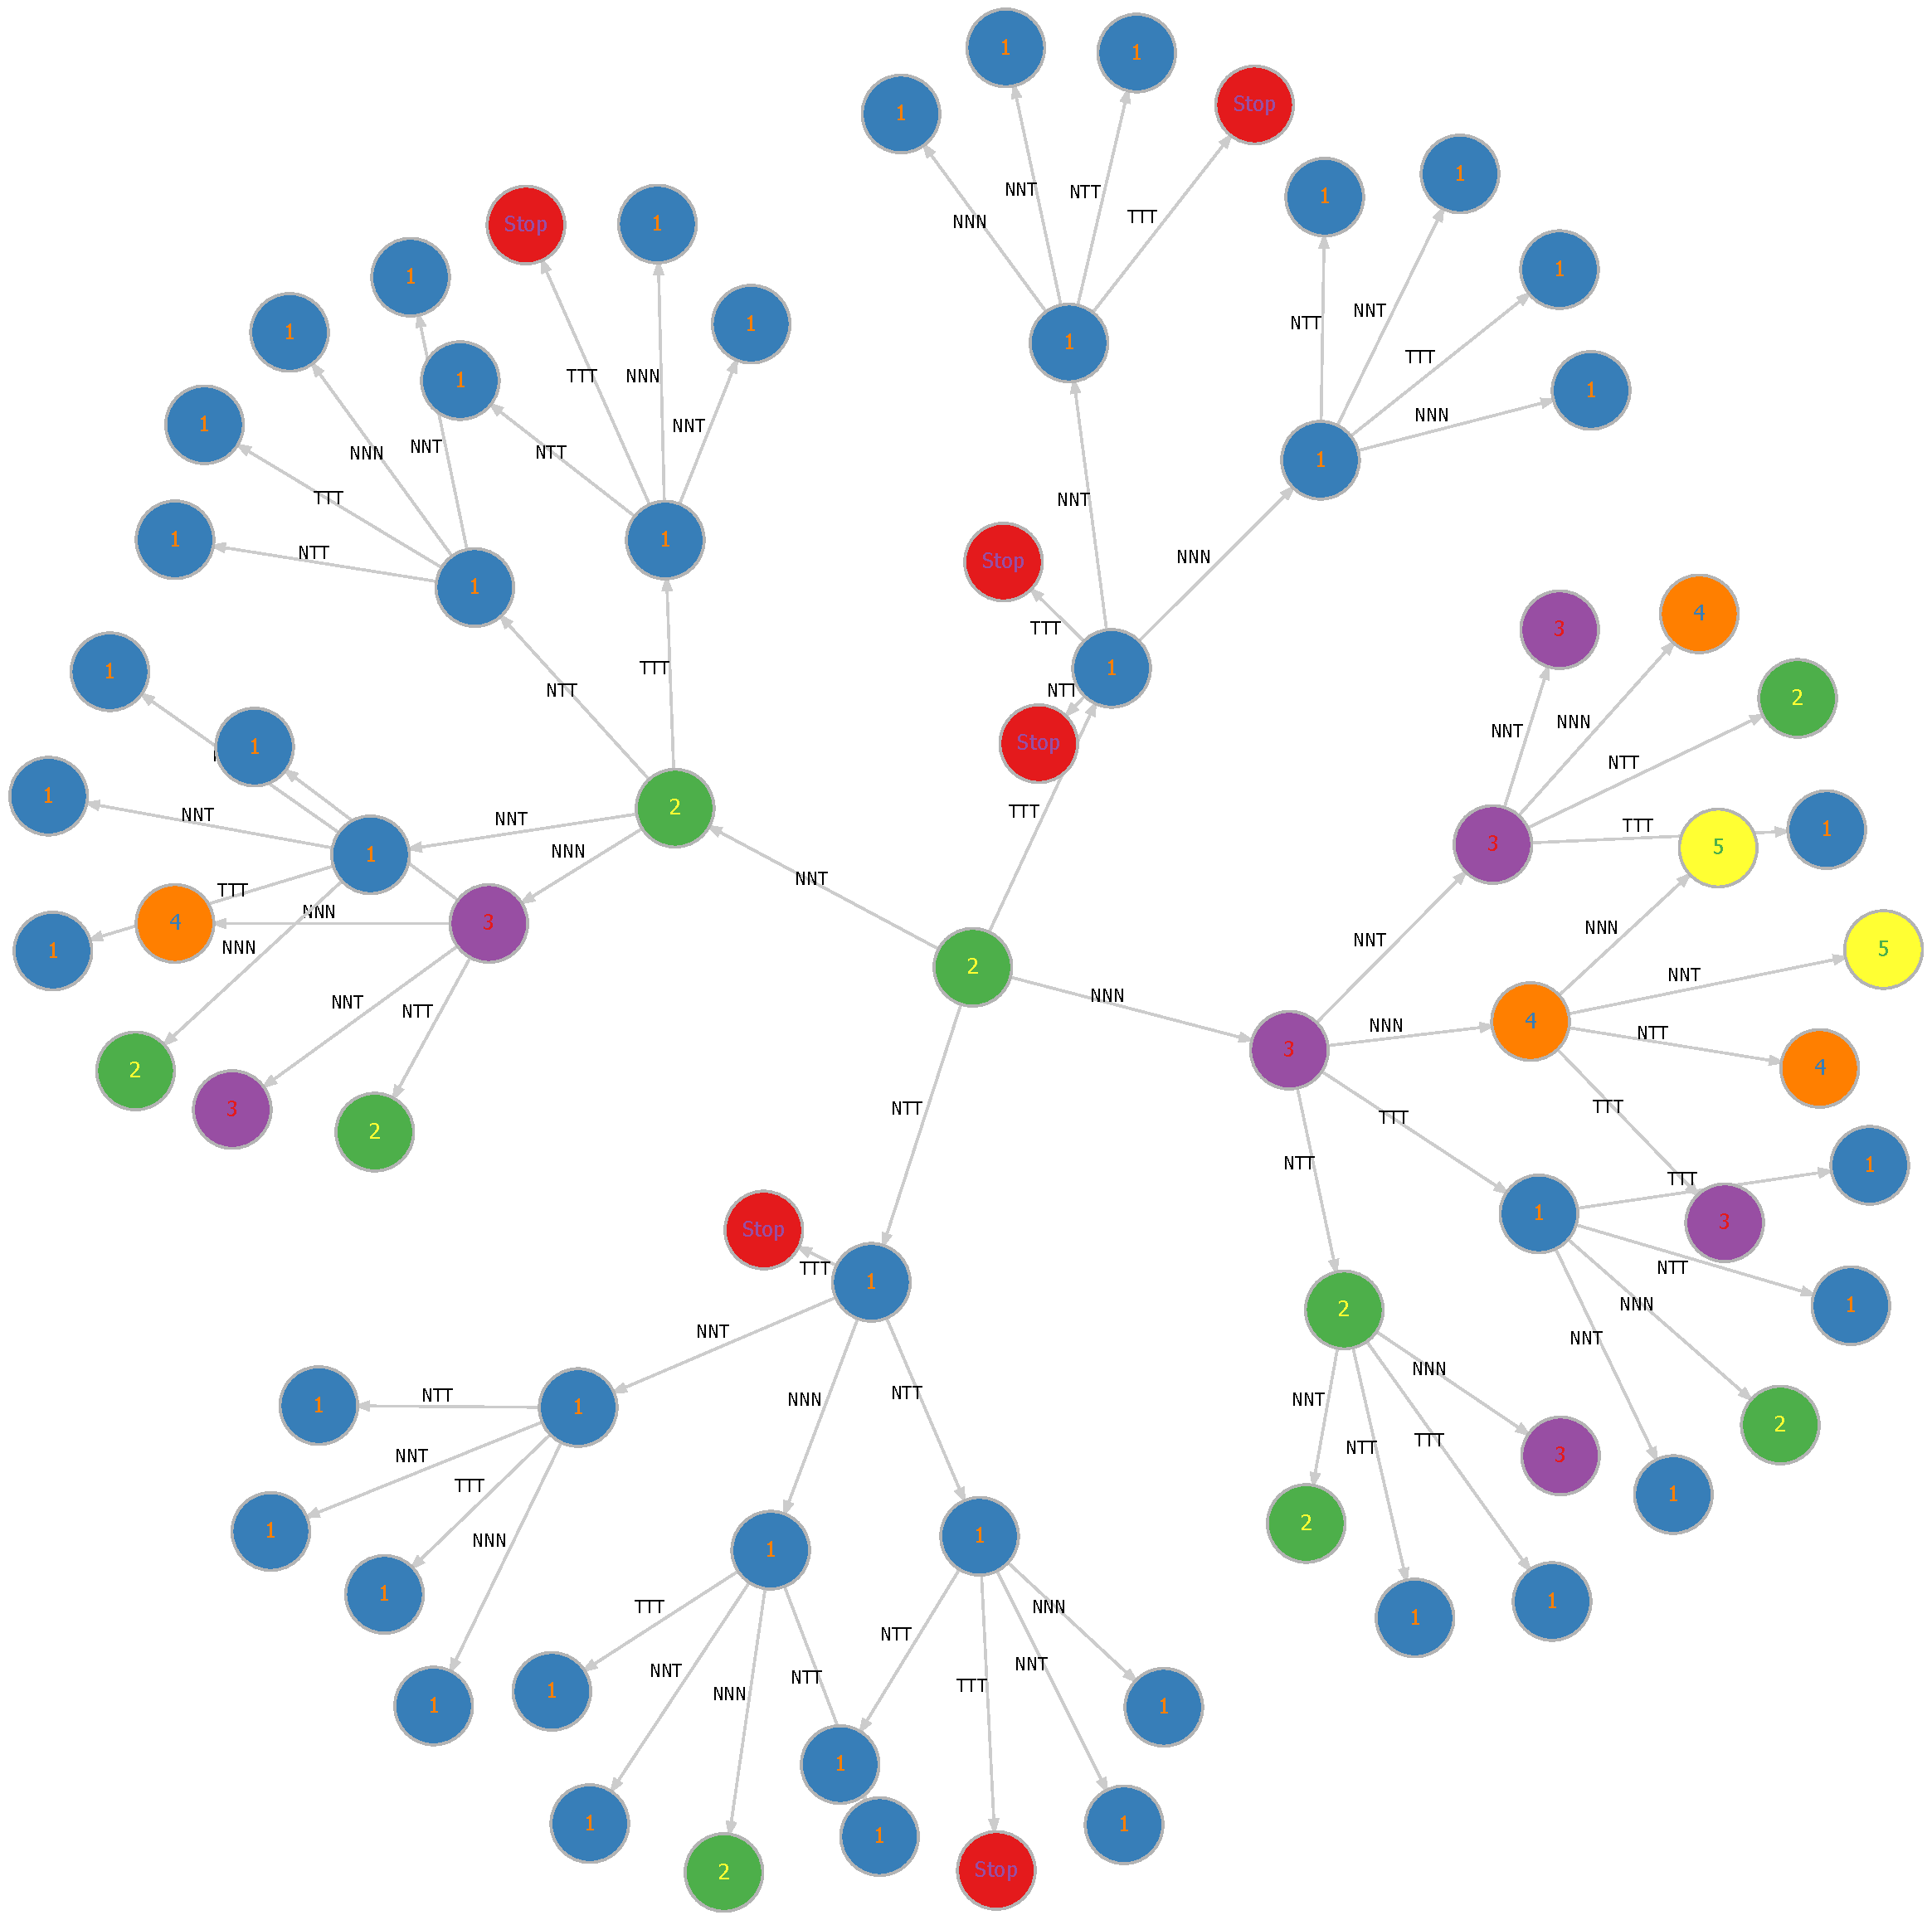
\includegraphics[width=\textwidth]{TITE-DTP-UpdatedExampleDTPNode}
\end{figure}

\begin{figure}[h!]
	\centering
	\caption[Updated DTP flow plot.]{Node plot of the updated DTP for the first two cohorts of our example CRM with additional rules.}
	\label{fig_tite-dtp:UpdatedDTPExampleFlow}
	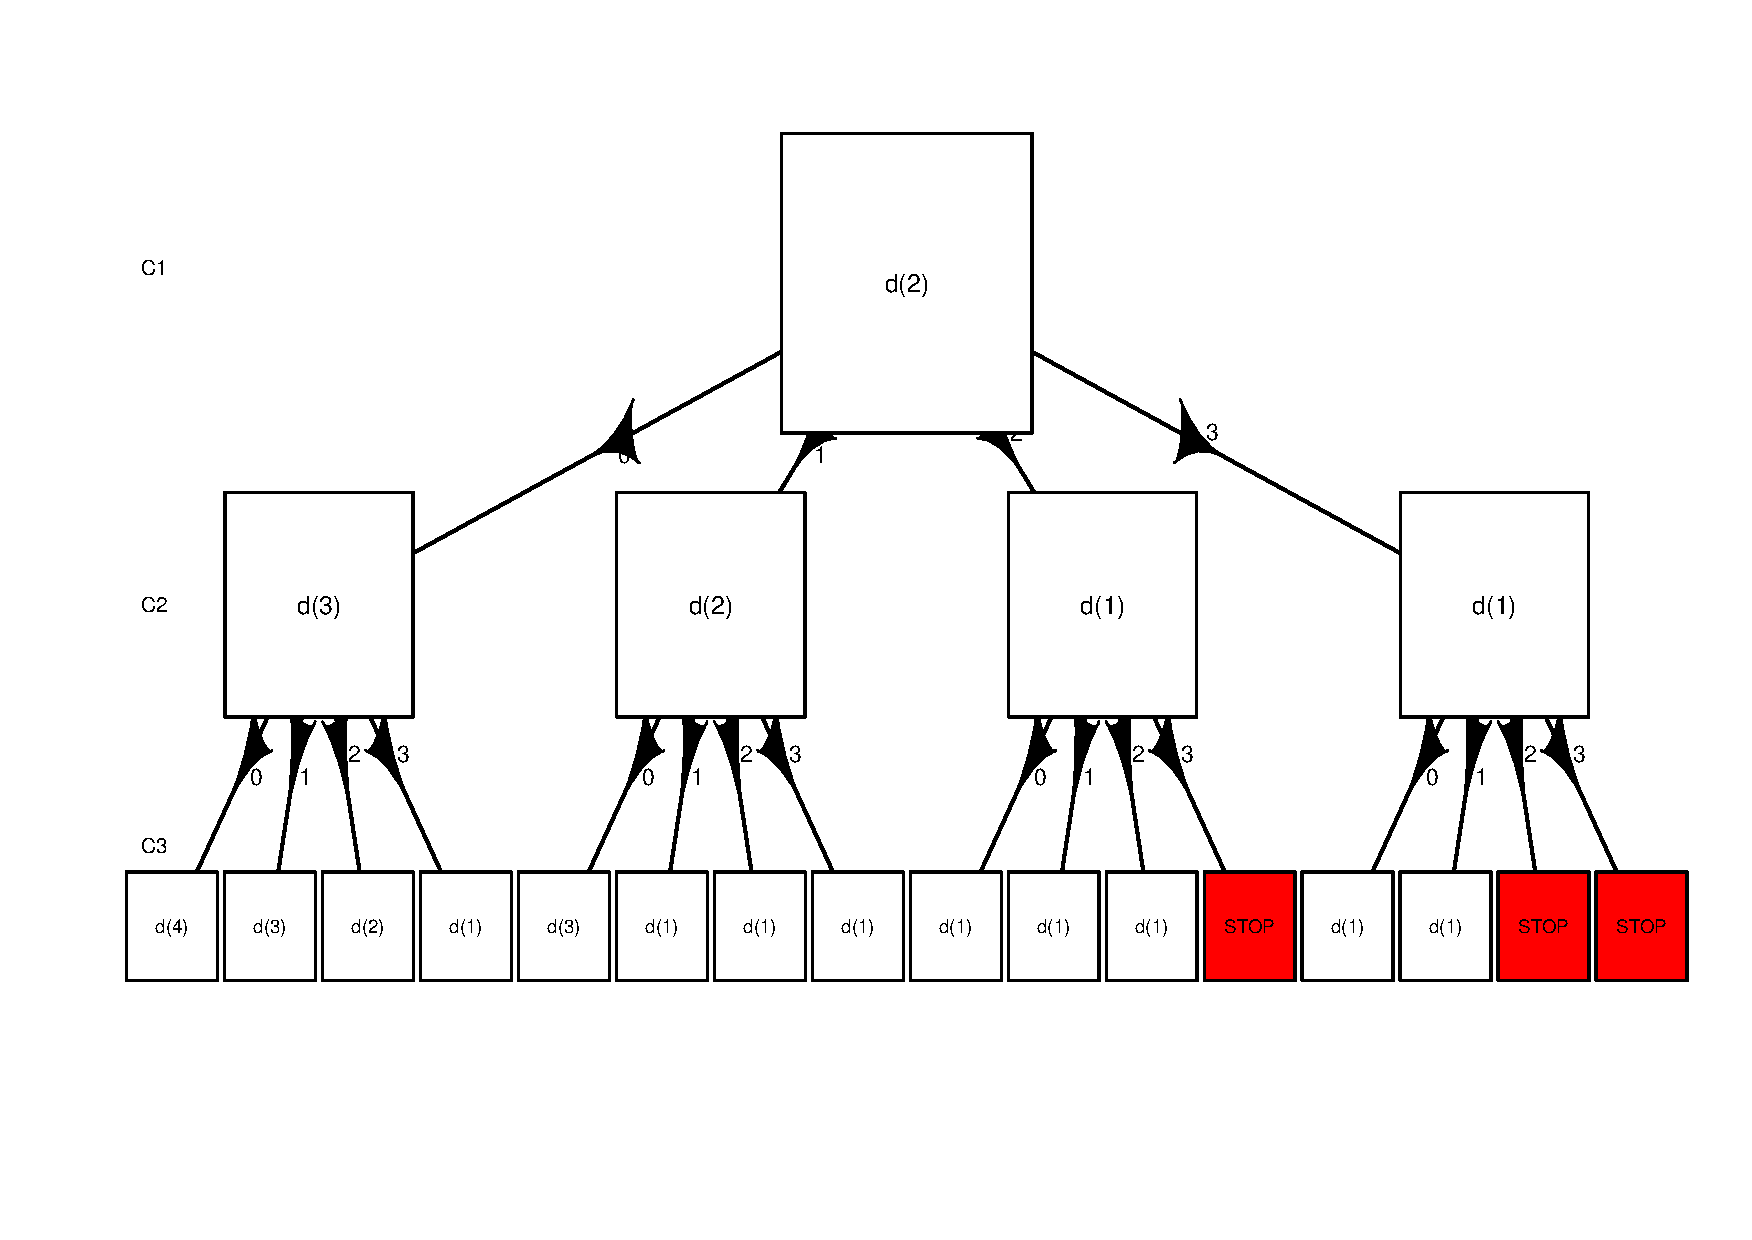
\includegraphics[width=\textwidth]{TITE-DTP-UpdatedExampleDTPFlow}
\end{figure}

At this stage, further discussions could be held about the updated DTPs and simulations. Here there, may be more subtle points to discuss such as the parameters of the stopping rule. Dependent on the clinical rational investigators may be inclined to impose either looser or stricter stopping rules. In our example here this can be done by altering the threshold values in our test of the posterior distribution of the probability of toxicity. 

We also see in pathway 2 that an escalation occurs after observing a toxicity in the previous cohort. This shows our design to be incoherent. A CRM design is considered coherent if escalation only occurs when the previous cohort experiences no DLTs and de-escalation only occurs when a DLT has been observed in the previous cohort. This property limits the risk of unnecessarily exposing patients to toxic doses whilst also ensuring patients get treated at a reasonable dose within the safety limit \cite{cheungDoseFindingContinual2011}. This became an issue due to the rule we enforced not to skip doses in escalation, the previous design without this rule was in fact coherent. Further rules could be added to ensure the design remains coherent such that escalation will only take place if the previous cohort experience no DLTs likewise, de-escalation will only occur if the previous cohort did experience DLTs. 

Here we have highlighted the ways in which DTPs can be utilised during the initial stages of setting up a trial. Due to our example there we some obvious changes that could be implemented into our suggested design. However, this was just to illustrate what the pathways look like and how they can be used to facilitate discussions with the relevant clinicians and the trials team. Although we just looked at DTPs any changes being made to the design should also take into account results from the simulations. CRM designs may not be intuitively understood by clinicians but DTPs should help make them more accessible. Next we will look at how DTPs can be used during a trial.  
%-----------------------------------
%	SUBSECTION 2
%-----------------------------------

\subsection{Using DTPs during a trial}

Dependent on the size of the dose finding trial it will often be infeasible to present all the different pathways. In our example with only 30 patients there were approximately 1 million different pathways. Even if we could present this data reasonably trying to decipher it may not be a worthwhile endeavour. The reason for there being so many pathways is that we have to evaluate every possible outcome for all patients at the start of the trial. As the trial progresses we observe outcomes for each patient and thus the number of pathways is reduced. We can then present DTPs for future cohorts of patients once we have accrued the outcome data of previous cohorts. 

DTPs main use in the design stage is allowing you to see how the model behaves with certain data and we can see if escalation and stopping are occurring as expected. We can then also communicate more effectively with clinicians and investigators what our design is doing. So, once a dose-finding trial has been designed, we can continue using DTPs whilst we are accruing data to project in advance dose-decisions that may occur. This has the potential to reduce the involvement of a statistician in the running and operational side of the trial. Additionally, time between recruitment of cohorts could also be reduced if the next recommended dose is the same dose regardless of the outcomes observed in the current cohort. It also allows us, like in the design stage, to check that the model is still escalating and stopping as expected. Although at this time it may be more difficult to make changes to the design of the trial once it is underway. 

In order to see how this would work in practice we will use the same example as specified in Section \ref{tite-dtp:Example-DTPs} along with the stopping rule we introduced in \ref{tite-dtp:UsingDTPs-Calibration}. Essentially, the same design that was used to produce the DTPs in Table \ref{tab_tite-dtp:UpdatedDTPExample} and Figure \ref{fig_tite-dtp:UpdatedDTPExampleNode}. Lets assume that we actually run this trial and that we see outcomes for the first three cohorts that match pathway 6 in Table\ref{tab_tite-dtp:UpdatedDTPExample}. That's to say; the first cohort of patients is recruited to dose-level 2 and no toxicities are observed, cohort 2 is allocated to dose-level 3 where one toxicity is observed, then cohort 3 is allocated to dose-level 3 where again only one toxicity is observed and that leads the  model recommending dose-level 3 for cohort 4. In order to refer to previous cohorts outcomes we will use nomenclature introduced by Brock \cite{brockImplementingEffToxDosefinding2017}. Outcomes for patients either toxicity (T) or no toxicity (N) is strung behind a numeric dose-level. For instance 2TTN denotes a cohort of three patients that were allocated to dose-level 2, two of whom experienced toxicity and one who didn't. In our example, using pathway 6 from Table \ref{tab_tite-dtp:UpdatedDTPExample}, these outcomes can be denoted as 2NNN 3NNT 3NNT. In this scenario we are unsure about the toxicity of dose-level 3 as we have seen toxicities in two separate cohorts, however this is mainly due to only having recruited 3 cohorts. If we consider this our new starting point we can produce new DTPs with these previous outcomes in mind. 

Table \ref{tab_tite-dtp:UsingDuringTrialDTPs4-7} shows the new set of DTPs following previous outcomes (2NNN 3NNT 3NNT), these are also visualised in Figure \ref{fig_tite-dtp:UsingDuringTrialDTPNode4-7}. For each pathway cohort 4 patients start at dose-level 3 as this is the model recommendation based on the previously observed outcomes. We have 64 pathways again which indicates that regardless of how many toxicities are observed the trial does not recommend stopping. See pathway 64, three patients have a toxicity at dose-level 3 then six have toxicities at dose-level 1. This doesn't necessarily mean that stopping rule isn't working as intended rather that due to the non-toxicities observed in the first three cohorts there would need to be more toxicity events before the rule we specified is triggered. This could be investigated further by looking at the DTPs following the outcomes of pathway 64 (i.e 2NNN 3NNT 3NNT 3TTT 1TTT 1TTT). It can also be seen if there are 2 or more toxicities we de-escalate and if there are no toxicities we escalate. There are also only 4 pathways where we end up at a higher dose at cohort 7 (pathways 1, 2, 5 and 17). Given the data we've already observed and if another toxicity occurs in cohort 4 there would need to be two cohorts of no toxicities before escalation can take place (pathway 17). 


\begin{table}[H]
	
	\caption{\label{tab_tite-dtp:UsingDuringTrialDTPs4-7}DTPs for three additional cohorts after observing outcomes for the first three cohorts.}
	\centering
	\resizebox{\linewidth}{!}{
		\fontsize{4}{3}\selectfont
		\begin{tabular}[t]{cccccccc}
			\toprule
			\multicolumn{1}{c}{} & \multicolumn{2}{c}{Cohort 4} & \multicolumn{2}{c}{Cohort 5} & \multicolumn{2}{c}{Cohort 6} & \multicolumn{1}{c}{Cohort 7} \\
			\cmidrule(l{3pt}r{3pt}){2-3} \cmidrule(l{3pt}r{3pt}){4-5} \cmidrule(l{3pt}r{3pt}){6-7} \cmidrule(l{3pt}r{3pt}){8-8}
			Pathway & Dose & Outcomes & Dose & Outcomes & Dose & Outcomes & Dose\\
			\midrule
			\cellcolor{gray!6}{1} & \cellcolor{gray!6}{3} & \cellcolor{gray!6}{NNN} & \cellcolor{gray!6}{4} & \cellcolor{gray!6}{NNN} & \cellcolor{gray!6}{4} & \cellcolor{gray!6}{NNN} & \cellcolor{gray!6}{5}\\
			2 & 3 & NNN & 4 & NNN & 4 & NNT & 4\\
			\cellcolor{gray!6}{3} & \cellcolor{gray!6}{3} & \cellcolor{gray!6}{NNN} & \cellcolor{gray!6}{4} & \cellcolor{gray!6}{NNN} & \cellcolor{gray!6}{4} & \cellcolor{gray!6}{NTT} & \cellcolor{gray!6}{3}\\
			4 & 3 & NNN & 4 & NNN & 4 & TTT & 3\\
			\cellcolor{gray!6}{5} & \cellcolor{gray!6}{3} & \cellcolor{gray!6}{NNN} & \cellcolor{gray!6}{4} & \cellcolor{gray!6}{NNT} & \cellcolor{gray!6}{4} & \cellcolor{gray!6}{NNN} & \cellcolor{gray!6}{4}\\
			6 & 3 & NNN & 4 & NNT & 4 & NNT & 3\\
			\cellcolor{gray!6}{7} & \cellcolor{gray!6}{3} & \cellcolor{gray!6}{NNN} & \cellcolor{gray!6}{4} & \cellcolor{gray!6}{NNT} & \cellcolor{gray!6}{4} & \cellcolor{gray!6}{NTT} & \cellcolor{gray!6}{3}\\
			8 & 3 & NNN & 4 & NNT & 4 & TTT & 3\\
			\cellcolor{gray!6}{9} & \cellcolor{gray!6}{3} & \cellcolor{gray!6}{NNN} & \cellcolor{gray!6}{4} & \cellcolor{gray!6}{NTT} & \cellcolor{gray!6}{3} & \cellcolor{gray!6}{NNN} & \cellcolor{gray!6}{3}\\
			10 & 3 & NNN & 4 & NTT & 3 & NNT & 3\\
			\cellcolor{gray!6}{11} & \cellcolor{gray!6}{3} & \cellcolor{gray!6}{NNN} & \cellcolor{gray!6}{4} & \cellcolor{gray!6}{NTT} & \cellcolor{gray!6}{3} & \cellcolor{gray!6}{NTT} & \cellcolor{gray!6}{2}\\
			12 & 3 & NNN & 4 & NTT & 3 & TTT & 2\\
			\cellcolor{gray!6}{13} & \cellcolor{gray!6}{3} & \cellcolor{gray!6}{NNN} & \cellcolor{gray!6}{4} & \cellcolor{gray!6}{TTT} & \cellcolor{gray!6}{2} & \cellcolor{gray!6}{NNN} & \cellcolor{gray!6}{3}\\
			14 & 3 & NNN & 4 & TTT & 2 & NNT & 2\\
			\cellcolor{gray!6}{15} & \cellcolor{gray!6}{3} & \cellcolor{gray!6}{NNN} & \cellcolor{gray!6}{4} & \cellcolor{gray!6}{TTT} & \cellcolor{gray!6}{2} & \cellcolor{gray!6}{NTT} & \cellcolor{gray!6}{2}\\
			16 & 3 & NNN & 4 & TTT & 2 & TTT & 1\\
			\cellcolor{gray!6}{17} & \cellcolor{gray!6}{3} & \cellcolor{gray!6}{NNT} & \cellcolor{gray!6}{3} & \cellcolor{gray!6}{NNN} & \cellcolor{gray!6}{3} & \cellcolor{gray!6}{NNN} & \cellcolor{gray!6}{4}\\
			18 & 3 & NNT & 3 & NNN & 3 & NNT & 3\\
			\cellcolor{gray!6}{19} & \cellcolor{gray!6}{3} & \cellcolor{gray!6}{NNT} & \cellcolor{gray!6}{3} & \cellcolor{gray!6}{NNN} & \cellcolor{gray!6}{3} & \cellcolor{gray!6}{NTT} & \cellcolor{gray!6}{3}\\
			20 & 3 & NNT & 3 & NNN & 3 & TTT & 2\\
			\cellcolor{gray!6}{21} & \cellcolor{gray!6}{3} & \cellcolor{gray!6}{NNT} & \cellcolor{gray!6}{3} & \cellcolor{gray!6}{NNT} & \cellcolor{gray!6}{3} & \cellcolor{gray!6}{NNN} & \cellcolor{gray!6}{3}\\
			22 & 3 & NNT & 3 & NNT & 3 & NNT & 3\\
			\cellcolor{gray!6}{23} & \cellcolor{gray!6}{3} & \cellcolor{gray!6}{NNT} & \cellcolor{gray!6}{3} & \cellcolor{gray!6}{NNT} & \cellcolor{gray!6}{3} & \cellcolor{gray!6}{NTT} & \cellcolor{gray!6}{2}\\
			24 & 3 & NNT & 3 & NNT & 3 & TTT & 2\\
			\cellcolor{gray!6}{25} & \cellcolor{gray!6}{3} & \cellcolor{gray!6}{NNT} & \cellcolor{gray!6}{3} & \cellcolor{gray!6}{NTT} & \cellcolor{gray!6}{2} & \cellcolor{gray!6}{NNN} & \cellcolor{gray!6}{3}\\
			26 & 3 & NNT & 3 & NTT & 2 & NNT & 2\\
			\cellcolor{gray!6}{27} & \cellcolor{gray!6}{3} & \cellcolor{gray!6}{NNT} & \cellcolor{gray!6}{3} & \cellcolor{gray!6}{NTT} & \cellcolor{gray!6}{2} & \cellcolor{gray!6}{NTT} & \cellcolor{gray!6}{1}\\
			28 & 3 & NNT & 3 & NTT & 2 & TTT & 1\\
			\cellcolor{gray!6}{29} & \cellcolor{gray!6}{3} & \cellcolor{gray!6}{NNT} & \cellcolor{gray!6}{3} & \cellcolor{gray!6}{TTT} & \cellcolor{gray!6}{2} & \cellcolor{gray!6}{NNN} & \cellcolor{gray!6}{2}\\
			30 & 3 & NNT & 3 & TTT & 2 & NNT & 1\\
			\cellcolor{gray!6}{31} & \cellcolor{gray!6}{3} & \cellcolor{gray!6}{NNT} & \cellcolor{gray!6}{3} & \cellcolor{gray!6}{TTT} & \cellcolor{gray!6}{2} & \cellcolor{gray!6}{NTT} & \cellcolor{gray!6}{1}\\
			32 & 3 & NNT & 3 & TTT & 2 & TTT & 1\\
			\cellcolor{gray!6}{33} & \cellcolor{gray!6}{3} & \cellcolor{gray!6}{NTT} & \cellcolor{gray!6}{2} & \cellcolor{gray!6}{NNN} & \cellcolor{gray!6}{3} & \cellcolor{gray!6}{NNN} & \cellcolor{gray!6}{3}\\
			34 & 3 & NTT & 2 & NNN & 3 & NNT & 3\\
			\cellcolor{gray!6}{35} & \cellcolor{gray!6}{3} & \cellcolor{gray!6}{NTT} & \cellcolor{gray!6}{2} & \cellcolor{gray!6}{NNN} & \cellcolor{gray!6}{3} & \cellcolor{gray!6}{NTT} & \cellcolor{gray!6}{2}\\
			36 & 3 & NTT & 2 & NNN & 3 & TTT & 2\\
			\cellcolor{gray!6}{37} & \cellcolor{gray!6}{3} & \cellcolor{gray!6}{NTT} & \cellcolor{gray!6}{2} & \cellcolor{gray!6}{NNT} & \cellcolor{gray!6}{2} & \cellcolor{gray!6}{NNN} & \cellcolor{gray!6}{2}\\
			38 & 3 & NTT & 2 & NNT & 2 & NNT & 2\\
			\cellcolor{gray!6}{39} & \cellcolor{gray!6}{3} & \cellcolor{gray!6}{NTT} & \cellcolor{gray!6}{2} & \cellcolor{gray!6}{NNT} & \cellcolor{gray!6}{2} & \cellcolor{gray!6}{NTT} & \cellcolor{gray!6}{1}\\
			40 & 3 & NTT & 2 & NNT & 2 & TTT & 1\\
			\cellcolor{gray!6}{41} & \cellcolor{gray!6}{3} & \cellcolor{gray!6}{NTT} & \cellcolor{gray!6}{2} & \cellcolor{gray!6}{NTT} & \cellcolor{gray!6}{1} & \cellcolor{gray!6}{NNN} & \cellcolor{gray!6}{2}\\
			42 & 3 & NTT & 2 & NTT & 1 & NNT & 1\\
			\cellcolor{gray!6}{43} & \cellcolor{gray!6}{3} & \cellcolor{gray!6}{NTT} & \cellcolor{gray!6}{2} & \cellcolor{gray!6}{NTT} & \cellcolor{gray!6}{1} & \cellcolor{gray!6}{NTT} & \cellcolor{gray!6}{1}\\
			44 & 3 & NTT & 2 & NTT & 1 & TTT & 1\\
			\cellcolor{gray!6}{45} & \cellcolor{gray!6}{3} & \cellcolor{gray!6}{NTT} & \cellcolor{gray!6}{2} & \cellcolor{gray!6}{TTT} & \cellcolor{gray!6}{1} & \cellcolor{gray!6}{NNN} & \cellcolor{gray!6}{1}\\
			46 & 3 & NTT & 2 & TTT & 1 & NNT & 1\\
			\cellcolor{gray!6}{47} & \cellcolor{gray!6}{3} & \cellcolor{gray!6}{NTT} & \cellcolor{gray!6}{2} & \cellcolor{gray!6}{TTT} & \cellcolor{gray!6}{1} & \cellcolor{gray!6}{NTT} & \cellcolor{gray!6}{1}\\
			48 & 3 & NTT & 2 & TTT & 1 & TTT & 1\\
			\cellcolor{gray!6}{49} & \cellcolor{gray!6}{3} & \cellcolor{gray!6}{TTT} & \cellcolor{gray!6}{1} & \cellcolor{gray!6}{NNN} & \cellcolor{gray!6}{2} & \cellcolor{gray!6}{NNN} & \cellcolor{gray!6}{2}\\
			50 & 3 & TTT & 1 & NNN & 2 & NNT & 2\\
			\cellcolor{gray!6}{51} & \cellcolor{gray!6}{3} & \cellcolor{gray!6}{TTT} & \cellcolor{gray!6}{1} & \cellcolor{gray!6}{NNN} & \cellcolor{gray!6}{2} & \cellcolor{gray!6}{NTT} & \cellcolor{gray!6}{1}\\
			52 & 3 & TTT & 1 & NNN & 2 & TTT & 1\\
			\cellcolor{gray!6}{53} & \cellcolor{gray!6}{3} & \cellcolor{gray!6}{TTT} & \cellcolor{gray!6}{1} & \cellcolor{gray!6}{NNT} & \cellcolor{gray!6}{1} & \cellcolor{gray!6}{NNN} & \cellcolor{gray!6}{2}\\
			54 & 3 & TTT & 1 & NNT & 1 & NNT & 1\\
			\cellcolor{gray!6}{55} & \cellcolor{gray!6}{3} & \cellcolor{gray!6}{TTT} & \cellcolor{gray!6}{1} & \cellcolor{gray!6}{NNT} & \cellcolor{gray!6}{1} & \cellcolor{gray!6}{NTT} & \cellcolor{gray!6}{1}\\
			56 & 3 & TTT & 1 & NNT & 1 & TTT & 1\\
			\cellcolor{gray!6}{57} & \cellcolor{gray!6}{3} & \cellcolor{gray!6}{TTT} & \cellcolor{gray!6}{1} & \cellcolor{gray!6}{NTT} & \cellcolor{gray!6}{1} & \cellcolor{gray!6}{NNN} & \cellcolor{gray!6}{1}\\
			58 & 3 & TTT & 1 & NTT & 1 & NNT & 1\\
			\cellcolor{gray!6}{59} & \cellcolor{gray!6}{3} & \cellcolor{gray!6}{TTT} & \cellcolor{gray!6}{1} & \cellcolor{gray!6}{NTT} & \cellcolor{gray!6}{1} & \cellcolor{gray!6}{NTT} & \cellcolor{gray!6}{1}\\
			60 & 3 & TTT & 1 & NTT & 1 & TTT & 1\\
			\cellcolor{gray!6}{61} & \cellcolor{gray!6}{3} & \cellcolor{gray!6}{TTT} & \cellcolor{gray!6}{1} & \cellcolor{gray!6}{TTT} & \cellcolor{gray!6}{1} & \cellcolor{gray!6}{NNN} & \cellcolor{gray!6}{1}\\
			62 & 3 & TTT & 1 & TTT & 1 & NNT & 1\\
			\cellcolor{gray!6}{63} & \cellcolor{gray!6}{3} & \cellcolor{gray!6}{TTT} & \cellcolor{gray!6}{1} & \cellcolor{gray!6}{TTT} & \cellcolor{gray!6}{1} & \cellcolor{gray!6}{NTT} & \cellcolor{gray!6}{1}\\
			64 & 3 & TTT & 1 & TTT & 1 & TTT & 1\\
			\bottomrule
	\end{tabular}}
\end{table}

\begin{figure}[h!]
	\centering
	\caption[DTP node plot for three additional cohorts.]{Node plot of three additional cohorts after observing outcomes for the first three cohorts.}
	\label{fig_tite-dtp:UsingDuringTrialDTPNode4-7}
	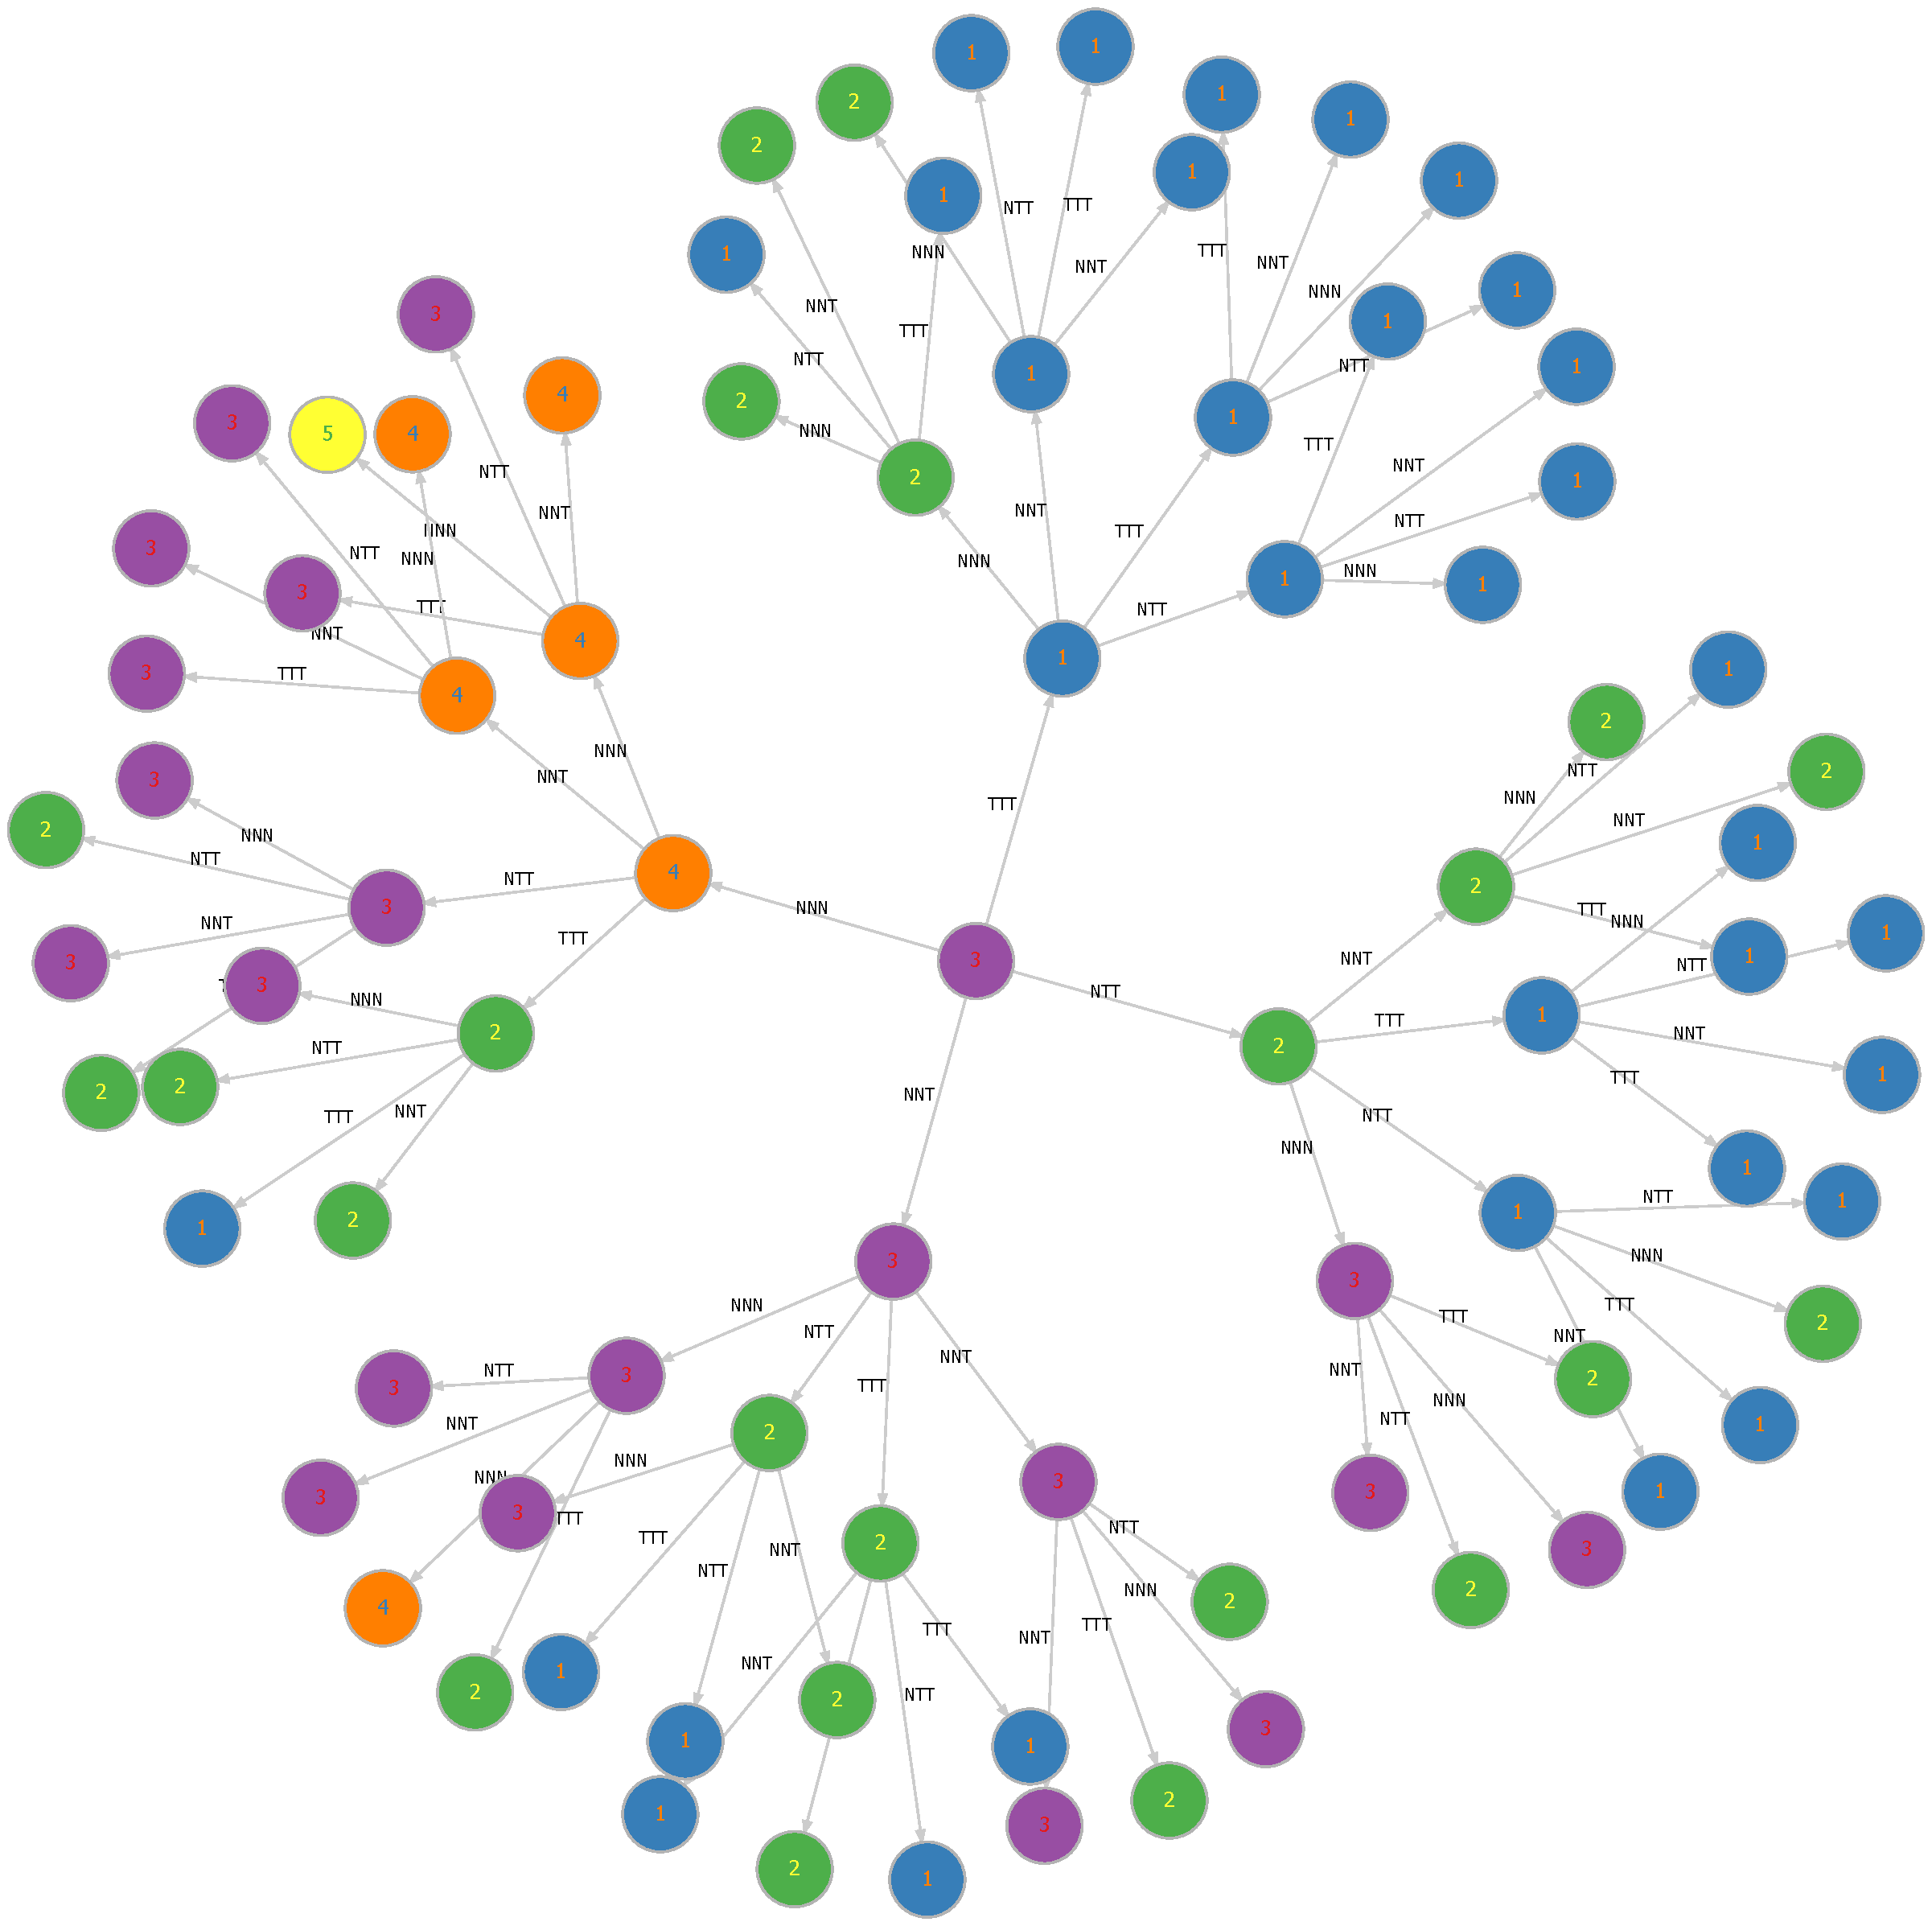
\includegraphics[width=\textwidth]{TITE-DTP-UsingDuringTrialDTPNode}
\end{figure}

Once cohort 7 is reached in the trial the DTPs can be updated again using the observed outcomes of whichever pathway occurred. These will show the potential pathways up to the 10th cohort, which is the maximum sample size in our example, and will also detail the final dose-recommendation. Throughout the trial the DTPs allow us to map out what doses are recommended all the way until the final decision. However, this has to be an iterative process as all the pathways can't be displayed simultaneously and  outcome data has to be accrued. 

DTPs can also work with non-uniform cohorts. So far our examples have been fairly simple however, in practice there may be complications with running a dose-finding trial. For instance there may be issues with recruitment leading to long time periods between the evaluation of cohorts and dose-decisions. This may be due to a number of factors such as lack of recruiting sites, underestimation of the prevalence of disease in the patient population or a global pandemic. One solution to this may be to reduce the cohort size and make dose-decisions earlier. Model-based designs are fairly flexible at dealing with issues like these as the model could just be updated after fewer patients instead. As these considerations may not have been made in the design stages of the trial DTPs could be used as a way to evaluate any changes to cohort sizes that are made during the trial. 

We will recreate the DTPs presented in this section except we will now use varying cohort sizes. These DTPs will use the same previously specified outcomes of 2NNN 3NNT 3NNT. DTPs will be calculated assuming the next three cohorts (cohorts 4,5 and 6) will only be able to recruit 2, 1 and 2 patients respectively. Table \ref{tab_tite-dtp:NonUniformDTPs4-7} lists the different pathways and they are also visualised in Figure \ref{fig_tite-dtp:NonUniformDTPNode4-7}. 

\begin{table}[H]
	
	\caption{\label{tab_tite-dtp:NonUniformDTPs4-7}DTPs for three additional cohorts with varying cohort sizes after observing outcomes for the first three cohorts.}
	\centering
	\resizebox{\linewidth}{!}{
		\fontsize{4}{3}\selectfont
		\begin{tabular}[t]{cccccccc}
			\toprule
			\multicolumn{1}{c}{} & \multicolumn{2}{c}{Cohort 4} & \multicolumn{2}{c}{Cohort 5} & \multicolumn{2}{c}{Cohort 6} & \multicolumn{1}{c}{Cohort 7} \\
			\cmidrule(l{3pt}r{3pt}){2-3} \cmidrule(l{3pt}r{3pt}){4-5} \cmidrule(l{3pt}r{3pt}){6-7} \cmidrule(l{3pt}r{3pt}){8-8}
			Pathway & Dose & Outcomes & Dose & Outcomes & Dose & Outcomes & Dose\\
			\midrule
			\cellcolor{gray!6}{1} & \cellcolor{gray!6}{3} & \cellcolor{gray!6}{NN} & \cellcolor{gray!6}{3} & \cellcolor{gray!6}{N} & \cellcolor{gray!6}{4} & \cellcolor{gray!6}{NN} & \cellcolor{gray!6}{4}\\
			2 & 3 & NN & 3 & N & 4 & NN & 4\\
			\cellcolor{gray!6}{3} & \cellcolor{gray!6}{3} & \cellcolor{gray!6}{NN} & \cellcolor{gray!6}{3} & \cellcolor{gray!6}{N} & \cellcolor{gray!6}{4} & \cellcolor{gray!6}{NT} & \cellcolor{gray!6}{3}\\
			4 & 3 & NN & 3 & N & 4 & NT & 3\\
			\cellcolor{gray!6}{5} & \cellcolor{gray!6}{3} & \cellcolor{gray!6}{NN} & \cellcolor{gray!6}{3} & \cellcolor{gray!6}{N} & \cellcolor{gray!6}{4} & \cellcolor{gray!6}{TT} & \cellcolor{gray!6}{3}\\
			6 & 3 & NN & 3 & N & 4 & TT & 3\\
			\cellcolor{gray!6}{7} & \cellcolor{gray!6}{3} & \cellcolor{gray!6}{NN} & \cellcolor{gray!6}{3} & \cellcolor{gray!6}{T} & \cellcolor{gray!6}{3} & \cellcolor{gray!6}{NN} & \cellcolor{gray!6}{3}\\
			8 & 3 & NN & 3 & T & 3 & NN & 3\\
			\cellcolor{gray!6}{9} & \cellcolor{gray!6}{3} & \cellcolor{gray!6}{NN} & \cellcolor{gray!6}{3} & \cellcolor{gray!6}{T} & \cellcolor{gray!6}{3} & \cellcolor{gray!6}{NT} & \cellcolor{gray!6}{2}\\
			10 & 3 & NN & 3 & T & 3 & NT & 2\\
			\cellcolor{gray!6}{11} & \cellcolor{gray!6}{3} & \cellcolor{gray!6}{NN} & \cellcolor{gray!6}{3} & \cellcolor{gray!6}{T} & \cellcolor{gray!6}{3} & \cellcolor{gray!6}{TT} & \cellcolor{gray!6}{2}\\
			12 & 3 & NN & 3 & T & 3 & TT & 2\\
			\cellcolor{gray!6}{13} & \cellcolor{gray!6}{3} & \cellcolor{gray!6}{NT} & \cellcolor{gray!6}{3} & \cellcolor{gray!6}{N} & \cellcolor{gray!6}{3} & \cellcolor{gray!6}{NN} & \cellcolor{gray!6}{3}\\
			14 & 3 & NT & 3 & N & 3 & NN & 3\\
			\cellcolor{gray!6}{15} & \cellcolor{gray!6}{3} & \cellcolor{gray!6}{NT} & \cellcolor{gray!6}{3} & \cellcolor{gray!6}{N} & \cellcolor{gray!6}{3} & \cellcolor{gray!6}{NT} & \cellcolor{gray!6}{2}\\
			16 & 3 & NT & 3 & N & 3 & NT & 2\\
			\cellcolor{gray!6}{17} & \cellcolor{gray!6}{3} & \cellcolor{gray!6}{NT} & \cellcolor{gray!6}{3} & \cellcolor{gray!6}{N} & \cellcolor{gray!6}{3} & \cellcolor{gray!6}{TT} & \cellcolor{gray!6}{2}\\
			18 & 3 & NT & 3 & N & 3 & TT & 2\\
			\cellcolor{gray!6}{19} & \cellcolor{gray!6}{3} & \cellcolor{gray!6}{NT} & \cellcolor{gray!6}{3} & \cellcolor{gray!6}{T} & \cellcolor{gray!6}{2} & \cellcolor{gray!6}{NN} & \cellcolor{gray!6}{2}\\
			20 & 3 & NT & 3 & T & 2 & NN & 2\\
			\cellcolor{gray!6}{21} & \cellcolor{gray!6}{3} & \cellcolor{gray!6}{NT} & \cellcolor{gray!6}{3} & \cellcolor{gray!6}{T} & \cellcolor{gray!6}{2} & \cellcolor{gray!6}{NT} & \cellcolor{gray!6}{2}\\
			22 & 3 & NT & 3 & T & 2 & NT & 2\\
			\cellcolor{gray!6}{23} & \cellcolor{gray!6}{3} & \cellcolor{gray!6}{NT} & \cellcolor{gray!6}{3} & \cellcolor{gray!6}{T} & \cellcolor{gray!6}{2} & \cellcolor{gray!6}{TT} & \cellcolor{gray!6}{1}\\
			24 & 3 & NT & 3 & T & 2 & TT & 1\\
			\cellcolor{gray!6}{25} & \cellcolor{gray!6}{3} & \cellcolor{gray!6}{TT} & \cellcolor{gray!6}{2} & \cellcolor{gray!6}{N} & \cellcolor{gray!6}{2} & \cellcolor{gray!6}{NN} & \cellcolor{gray!6}{2}\\
			26 & 3 & TT & 2 & N & 2 & NN & 2\\
			\cellcolor{gray!6}{27} & \cellcolor{gray!6}{3} & \cellcolor{gray!6}{TT} & \cellcolor{gray!6}{2} & \cellcolor{gray!6}{N} & \cellcolor{gray!6}{2} & \cellcolor{gray!6}{NT} & \cellcolor{gray!6}{2}\\
			28 & 3 & TT & 2 & N & 2 & NT & 2\\
			\cellcolor{gray!6}{29} & \cellcolor{gray!6}{3} & \cellcolor{gray!6}{TT} & \cellcolor{gray!6}{2} & \cellcolor{gray!6}{N} & \cellcolor{gray!6}{2} & \cellcolor{gray!6}{TT} & \cellcolor{gray!6}{1}\\
			30 & 3 & TT & 2 & N & 2 & TT & 1\\
			\cellcolor{gray!6}{31} & \cellcolor{gray!6}{3} & \cellcolor{gray!6}{TT} & \cellcolor{gray!6}{2} & \cellcolor{gray!6}{T} & \cellcolor{gray!6}{1} & \cellcolor{gray!6}{NN} & \cellcolor{gray!6}{2}\\
			32 & 3 & TT & 2 & T & 1 & NN & 2\\
			\cellcolor{gray!6}{33} & \cellcolor{gray!6}{3} & \cellcolor{gray!6}{TT} & \cellcolor{gray!6}{2} & \cellcolor{gray!6}{T} & \cellcolor{gray!6}{1} & \cellcolor{gray!6}{NT} & \cellcolor{gray!6}{1}\\
			34 & 3 & TT & 2 & T & 1 & NT & 1\\
			\cellcolor{gray!6}{35} & \cellcolor{gray!6}{3} & \cellcolor{gray!6}{TT} & \cellcolor{gray!6}{2} & \cellcolor{gray!6}{T} & \cellcolor{gray!6}{1} & \cellcolor{gray!6}{TT} & \cellcolor{gray!6}{1}\\
			36 & 3 & TT & 2 & T & 1 & TT & 1\\
			\bottomrule
	\end{tabular}}
\end{table}

\begin{figure}[h!]
	\centering
	\caption[DTP node plot for three additional various sized cohorts.]{Node plot of three additional cohorts with varying cohort sizes after observing outcomes for the first three cohorts.}
	\label{fig_tite-dtp:NonUniformDTPNode4-7}
	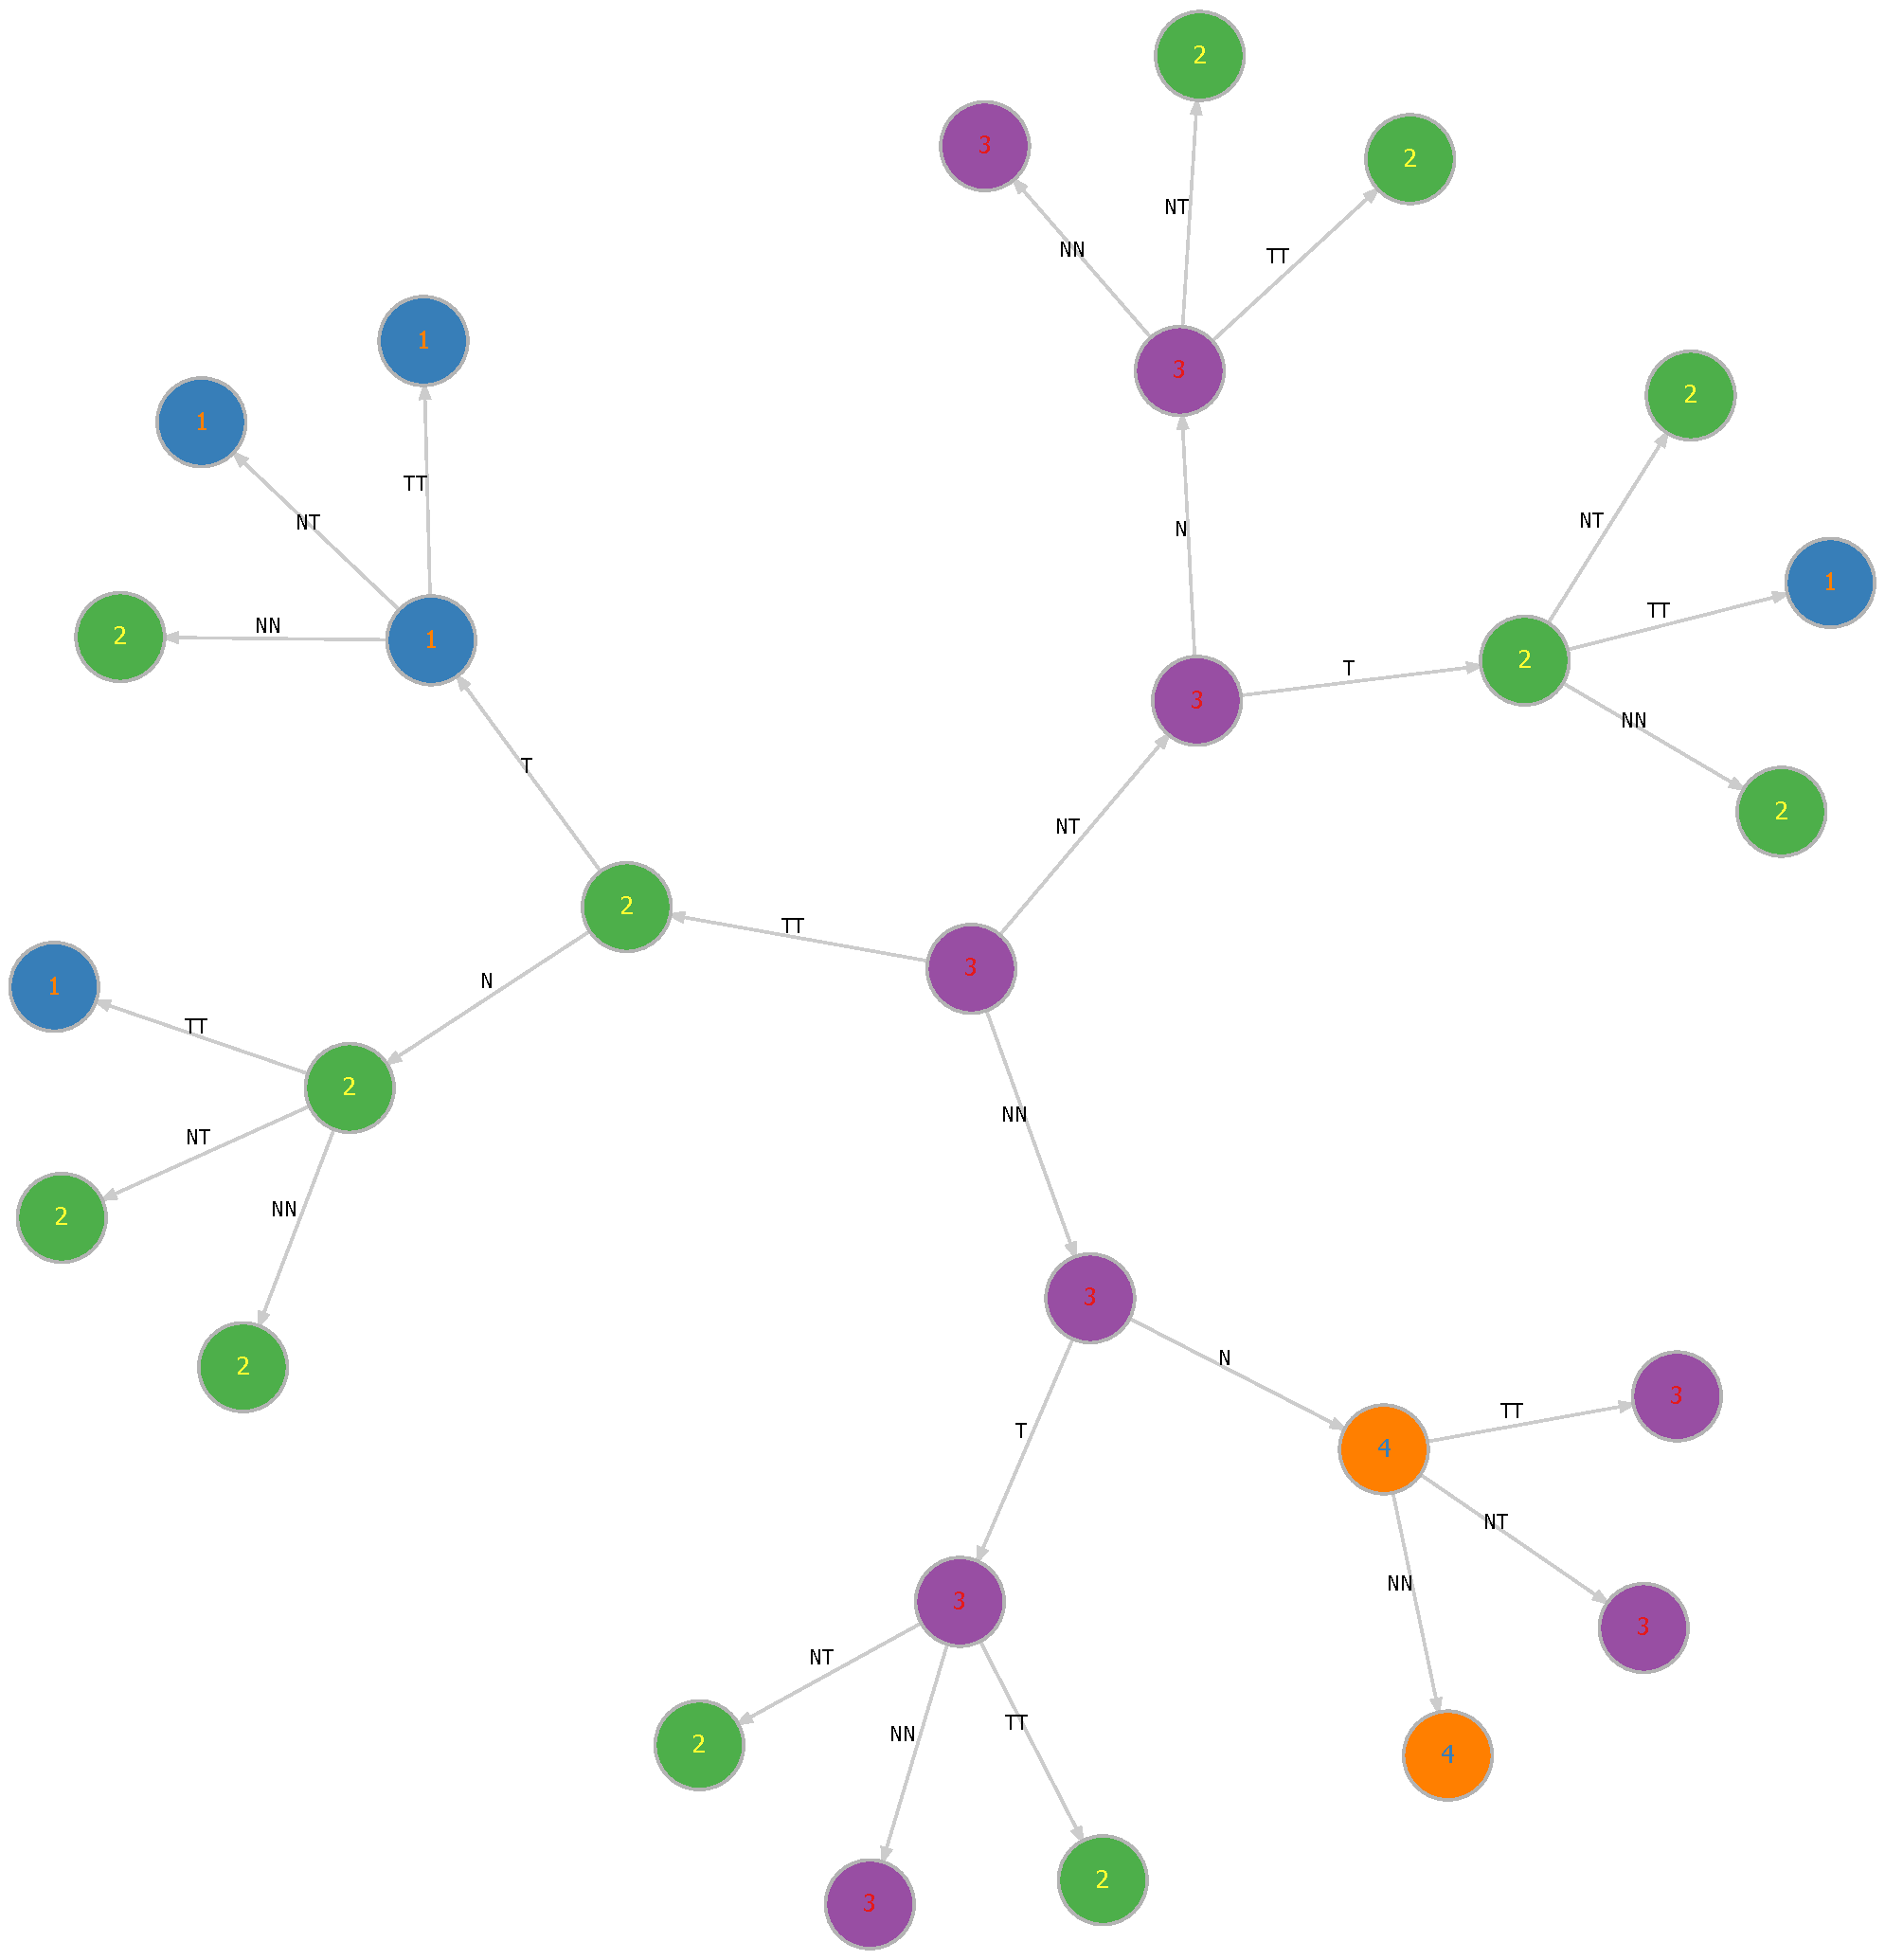
\includegraphics[width=\textwidth]{TITE-DTP-NonUniformDTPNode}
\end{figure}

These DTPs can be interpreted in the same way as before but now just correspond to a different number of patients. Where the recommended dose is set at dose-level 3 for cohort 5 we can consider these pathways equivalent to those presented earlier in Table \ref{tab_tite-dtp:UsingDuringTrialDTPs4-7} for cohort 4. As in oth of these scenarios 3 patients would have been treated at dose-level 3. For instance pathways 1-6 and its recommended dose for cohort 6 in Table \ref{tab_tite-dtp:NonUniformDTPs4-7} are equivalent to pathways 1-16 and its recommended dose for cohort 5 in Table \ref{tab_tite-dtp:UsingDuringTrialDTPs4-7}, This is because in both instances 3 patients have been treated at the same dose-level and all have the same outcome. Of course this does not always hold as a dose-decision made on less data may lead to a different dose-decision and hence create a different pathway. In the scenarios where two patients experience a toxicity the model de-escalates and since there isn't a third patient at that dose-level 3 the following pathways will all differ from those presented previously. 

We have established how DTPs can also be used not only during the design and calibration of a trial but also whilst it is running. They have the ability to communicate dose decisions effectively. They also help alleviate some of the potential mystery behind model based designs where clinicians and non-statisticians involved in trials may not appreciate how dose decisions are being made by a model such as the CRM. Additionally, they can also be used to assess any modifications that need to be made to the design due to practical or logistical issues. It is clear DTPs are a valuable tool to incorporate in any dose-finding trial and with the escalation package by Brock \cite{brockModularApproachDose2020} they are very easy to implement, only requiring a few lines of code. In the next section we explore the possibility of extending DTPs to work in the time-to-event setting.  

%----------------------------------------------------------------------------------------
%	SECTION 3
%----------------------------------------------------------------------------------------

\section{TiTE-DTPs}
\label{tite-dtp:TITE-DTPs}